\newcommand{\DoNotLoadEpstopdf}{}
\documentclass[11pt]{article}
\usepackage[T1]{fontenc}
\usepackage{lmodern}
\usepackage[margin=1in]{geometry}
\usepackage{amsmath,amssymb,amsthm,mathtools}
\usepackage{microtype,booktabs,array}
\usepackage{flafter}
\usepackage{tikz}
\usetikzlibrary{arrows.meta,calc}
\usepackage[colorlinks=true,linkcolor=blue!45!black,citecolor=blue!45!black,urlcolor=blue!45!black]{hyperref}
\hypersetup{pdftitle={Smooth isometric immersions of closed surfaces into Euclidean four-space},pdfauthor={OpenAI},pdfsubject={Smooth isometric immersions of closed Riemannian surfaces}}
\usepackage{enumitem}
\setlist{itemsep=2pt,topsep=5pt}
\newtheorem{theorem}{Theorem}[section]
\newtheorem{proposition}[theorem]{Proposition}
\newtheorem{lemma}[theorem]{Lemma}
\newtheorem{corollary}[theorem]{Corollary}
\theoremstyle{definition}
\newtheorem{definition}[theorem]{Definition}
\theoremstyle{remark}
\newtheorem{remark}[theorem]{Remark}
\numberwithin{equation}{section}
\newcommand{\R}{\mathbb{R}}
\newcommand{\avg}{\operatorname{avg}}
\newcommand{\supp}{\operatorname{supp}}
\newcommand{\Hess}{\operatorname{Hess}}
\newcommand{\Id}{\operatorname{Id}}
\newcommand{\Span}{\operatorname{span}}
\newcommand{\II}{\mathrm{II}}
\title{Smooth isometric immersions of closed surfaces\\into Euclidean four-space}
\author{OpenAI}
\date{September 23, 2026}
\begin{document}
\maketitle
\begin{abstract}
Every closed smooth Riemannian surface admits a smooth isometric immersion into
Euclidean four-space, without an orientability assumption. This resolves the
closed-surface form of the classical four-dimensional isometric-immersion problem.
\end{abstract}
\tableofcontents
\section{Introduction}\label{sec:introduction}

Let $M$ be a closed smooth surface: a compact smooth two-dimensional manifold
without boundary. We do not assume that $M$ is orientable or connected.
For a smooth positive definite metric $g$ on $M$, an isometric immersion into
Euclidean four-space is a smooth map $F:M\to\R^4$ satisfying
\[
 \langle dF_p(v),dF_p(w)\rangle=g_p(v,w)
 \qquad(p\in M,\ v,w\in T_pM).
\]
Positive definiteness then makes $dF_p$ injective at every point.
The question is whether every such metric can be realized in this dimension.

\begin{theorem}\label{thm:main}
Every closed smooth Riemannian surface $(M,g)$ admits a $C^\infty$ isometric
immersion into $(\R^4,\delta_4)$, where $\delta_4=\sum_{i=1}^4 dx_i^2$.
\end{theorem}

The result concerns immersion; self-intersections are allowed. There is no
restriction on Gaussian curvature or on the topology of the closed surface.
In particular, the construction applies directly to nonorientable surfaces.

\subsection{Context}
Gromov explicitly recorded the question of smooth isometric immersion of
arbitrary smooth Riemannian surfaces into $\R^4$
\cite[\S I, Remark~(d), p.~3 of the author version]{Gromov2000}.
He later attributed the four-space surface question to Chern around 1950,
while expressing uncertainty about the compactness qualification
\cite[p.~4, footnote~6]{Gromov2015}.
Theorem~\ref{thm:main} concerns the compact boundaryless case of this question.

Nash's smooth embedding theorem gives a global realization of a compact
$n$-dimensional Riemannian manifold in dimension $n(3n+11)/2$, which is $17$
for surfaces \cite[Theorem~2, p.~59]{Nash1956}.
A closer surface comparison is Gromov's construction of smooth
isometric immersions of closed surfaces into $\R^5$: his retrospective
explicitly recalls this result and refers to \S3.2.4 of
\emph{Partial Differential Relations}
\cite[p.~59]{Gromov2015}\cite{GromovPDR1986}.
Theorem~\ref{thm:main} lowers this immersion dimension to four.

The local analytic theory reaches a smaller dimension. The theorem of
Janet and Cartan places an analytic Riemannian surface locally and
isometrically in $\R^3$ \cite{Janet1926,Cartan1927}; see also the
formulation in \cite[\S1.2]{Gromov2015}.
Both the analytic hypothesis and the local conclusion matter here.
For comparison, the companion \cite[Theorem~A]{OpenAILocalObstruction2026}
constructs a smooth positive definite metric on $(-1,1)^2$ for which no
neighborhood of the origin admits a smooth isometric immersion into $\R^3$.

There is also a smooth four-dimensional theory on planar domains.
Poznyak proved that $C^{3,\alpha}$ data admit $C^{2,\alpha}$ isometric
immersions into $\R^4$ on compact portions of a simply connected planar
domain with regular boundary \cite[Theorem~4, p.~67]{Poznyak1973}.
The smooth version of this construction is stated and explained in
Lewicka's modern account \cite[Theorem~9.1, p.~57]{Lewicka2026v3}.
Passing from planar domains to a closed surface requires the corrections
to remain compatible through a global construction. Here we achieve this
by preserving the normal geometry needed for successive local metric
corrections.

Regularity gives a second distinction. An immersion is \emph{strictly short}
if the prescribed metric minus its induced metric is positive definite.
Nash's oscillatory construction and Kuiper's codimension-one refinement show
that a strictly short immersion in positive codimension can be uniformly
approximated by $C^1$ isometric
immersions \cite{Nash1954,Kuiper1955}; the contemporaneous account
\cite[Theorems~1--2]{Choquet1958} states the immersion form explicitly.
Lewicka proves a finer flexibility theorem in $\R^4$ for metrics of low
H\"older regularity. In the August 2026 version, the domain is bounded,
planar, and diffeomorphic to a disk, the metric is $C^{r,\beta}$ on its
closure with $0<r+\beta\le2$, and strictly short $C^1$ immersions admit
uniform approximation by $C^{1,\alpha}$ isometric immersions for
$0<\alpha<\min\{(r+\beta)/2,1\}$
\cite[Theorem~1.1, p.~2]{Lewicka2026v3}.
These domain and regularity hypotheses differ from the smooth
closed-surface statement of Theorem~\ref{thm:main}.

The proof uses the established ideas of positive rank-one metric
decomposition, oscillatory metric correction, and smoothing to control
derivative loss. We give the corresponding attribution where these ideas
enter the construction. The mode equations, finite correctors, smooth
convergence argument, and propagation of the normal geometry are proved
below. Whitney's ordinary immersion theorem supplies the starting map
\cite[Theorem~8, p.~274]{Whitney1944}; Sard's equal-dimensional
critical-value theorem is used to choose the support boundaries and phases
\cite[Theorem~4.1, p.~885]{Sard1942}.

\subsection{The construction}
The proof has four stages. First prepare a smooth immersion into a small round
three-sphere in $\R^4$ together with a finite decomposition of its metric
deficit. Its induced metric $g_0$ is strictly below $g$, and the negative
radial direction is a globally defined normal, including when $M$ is
nonorientable. The decomposition has the form
\begin{equation}\label{eq:intro-sum}
 g-g_0=\sum_{j=1}^{J_0} a_j^2\,dx_j^2,
\end{equation}
where each $x_j$ is a coordinate function on a disk and $a_j$ is smooth,
positive in that disk, and zero outside it. The decomposition is arranged so
that each phase has a positive transverse Hessian for the metric immediately
preceding its addition.

Second, let $F$ be the current immersion and consider one addition
$a^2dx^2$. Write $y$ for a complementary coordinate. The relevant plane is
perpendicular to both $F_y$ and $F_{yy}$.
A periodic path on a circle in this plane has the prescribed average and
adds $a^2dx^2$ to the leading metric. Orthogonality to $F_{yy}$ removes
the first transverse metric error. A finite expansion then cancels the
oscillatory errors to an arbitrarily prescribed order. Its remaining mean
terms form a finite differential perturbation of the induced-metric map.
Small corrections on a slower scale reduce this perturbed map's error to
the required finite accuracy.

Third, turn the resulting approximate metric into an exact one. We prove a
smooth correction theorem under the pointwise hypothesis that the
vector-valued second fundamental form is nonzero. A finite construction solves
the linearized equation on individual oscillatory modes to arbitrarily high
finite accuracy, with suitably chosen phase directions.
Smoothing between successive steps controls the lost derivatives; increasing
the accuracy in successive blocks gives convergence in every smooth norm.
No global inverse of the linearized metric map is required.

Finally, retain the geometric conditions needed for the remaining disks.
The large oscillation may rotate the second fundamental form. Conditions on
the later boundary curves, and a choice of large transverse derivatives at the
turns of the velocity loop, prevent its relevant normal directions from
vanishing or becoming opposite to the preferred normal. The small $C^2$ exact correction preserves the
required derivative asymptotics. Together with the exact Gauss equation,
these asymptotics establish the strict boundary and crossing conditions.
After the finite list of additions, the induced metric is $g$ by
\eqref{eq:intro-sum}.

The two analytical devices used here have separate roles. The small-mode
construction supplies high-order metric accuracy while its displacement is
small in $C^2$. The large circle construction changes the metric by a prescribed
positive primitive tensor while retaining selected second-derivative
information. Their combination is what permits a finite global construction
in codimension two.  The number of global primitive additions is finite;
within each addition, however, the exact correction uses an infinite
smoothing iteration converging to one map in every $C^m$ norm.

\subsection{Organization}
Section~\ref{sec:preliminaries} sets up normal geometry and admissible phases.
Section~\ref{sec:primitive-statement} states the primitive-addition theorem,
including the boundary conditions it preserves.
Sections~\ref{sec:small-modes} and~\ref{sec:exact-correction} prove the small
increment and exact correction results.
Sections~\ref{sec:velocity-loop} and~\ref{sec:primitive-realization} construct
the velocity loop and realize the primitive metric.
Section~\ref{sec:geometry-preservation} completes the primitive-addition proof.
Section~\ref{sec:global-construction} prepares the finite list and proves
Theorem~\ref{thm:main}.

\section{Normal geometry and admissible phases}\label{sec:preliminaries}

We begin with the geometric information used by both corrections. A nonzero
second fundamental form supplies enough directions for the small oscillations;
it need not satisfy any rank condition beyond being nonzero as a tensor.

Fix a smooth background metric and a finite collection of precompact coordinate
patches on $M$. All $C^m$ norms and unmarked tangent norms use these fixed data.
For a smooth immersion $F:M\to\R^4$, write
\[
 \gamma(F)=F^*\delta_4,
 \qquad N_F=(dF(TM))^\perp,
 \qquad B_F(V,W)=\operatorname{proj}_{N_F}D_V(dF(W)).
\]
The last expression is tensorial; in coordinates $B_{F,ij}$ is the normal
projection of $F_{ij}$. Let $K_\gamma$ denote the Gaussian curvature of
$\gamma=\gamma(F)$. Our sign convention for the Gauss equation is
\begin{equation}\label{eq:gauss}
 \langle B_F(V,V),B_F(W,W)\rangle-|B_F(V,W)|^2
 =K_\gamma\,|V\wedge W|_\gamma^2.
\end{equation}
In coordinates $x,y$, the right side is $K_\gamma\det\gamma$ for
$V=\partial_x,W=\partial_y$. The Hessian convention gives
$\Hess_\gamma x(\partial_y,\partial_y)=-\Gamma^x_{yy}$.
To check \eqref{eq:gauss}, choose Riemannian normal coordinates for
$\gamma$, orthonormal at the point under consideration.
There $\Gamma=0$, so $F_{xx},F_{xy},F_{yy}$ are normal vectors, and the
coordinate curvature formula is
\[
 K_\gamma=\partial_{xy}\gamma_{xy}
 -\tfrac12\bigl(\partial_{xx}\gamma_{yy}
                  +\partial_{yy}\gamma_{xx}\bigr).
\]
Substituting $\gamma_{ij}=\langle F_i,F_j\rangle$ cancels the third
derivatives and gives
$K_\gamma=\langle F_{xx},F_{yy}\rangle-|F_{xy}|^2$ at that point.
Tensoriality gives \eqref{eq:gauss} for arbitrary $V,W$.

A \emph{preferred normal} is a smooth unit section of $N_F$. This is less than a
normal frame: we will use complementary normal vectors only within coordinate
disks. None of the following local constructions requires an orientation of $M$.

\begin{definition}
A nonzero covector $\xi\in T_p^*M$ is \emph{good for $F$} if
$B_F(Y,Y)\ne0$ for a nonzero vector $Y\in\ker\xi$.
This condition is independent of the choice of $Y$ in that line.
\end{definition}

If $B_F(p)\ne0$, there are only finitely many bad projective covectors at $p$.
Indeed, take a normal component of $B_F(p)$ that is a nonzero scalar quadratic
form. Its zeros in the projective tangent line are finite, and a zero of the
vector-valued quadratic form must be one of these zeros.

We choose these good directions for the small oscillatory corrections.
They need not be the phases $x_j$ of the prescribed primitive additions in
\eqref{eq:intro-sum}: those phases will satisfy a transverse Hessian
condition, and their transverse second fundamental form may vanish in the
interior of the support disk.

Writing a positive metric as a sum of positive rank-one forms is a basic
part of Nash's construction \cite{Nash1954}; see
\cite[\S3.5.4, p.~32 and footnote~30]{Gromov2015} and
\cite[Lemmas~2.2--2.3]{Kallen1978} for related decompositions.
Here the individual phases and their relevant pairwise combinations must
also be good for the current second fundamental form.  The following
construction supplies those additional conditions.

\begin{lemma}[Positive phase decompositions]\label{lem:phase-data}
Let $F:M\to\R^4$ be a smooth immersion with $B_F(p)\ne0$ for every $p$, and let
$h_0$ be a smooth positive definite tensor. There are finitely many functions
$\phi_\nu$ defined on coordinate patches, smooth cutoffs $\psi_\nu$ supported
compactly in those patches, and smooth fiberwise linear forms $q_\nu$ on
symmetric tensors, such that
\begin{equation}\label{eq:phase-decomposition}
 H=\sum_\nu b_\nu(H)^2\,d\phi_\nu^2,
 \qquad b_\nu(H)=\psi_\nu\sqrt{q_\nu(H)}
\end{equation}
whenever $H$ is sufficiently close to $h_0$ in $C^0$. Every square root has a
strict positive lower bound before multiplication by the cutoff. On the
appropriate supports the differentials of $\phi_\nu$, $2\phi_\nu$, and
$\phi_\nu\pm\phi_\mu$ for $\nu\ne\mu$ are nonzero and good. These conclusions
persist for immersions in a sufficiently small $C^2$ neighborhood of $F$.
Each phase or phase combination has a smooth complementary coordinate
coframe on the support where it is used.
\end{lemma}

\begin{proof}
At a point choose an $h_0$-orthonormal coframe and three covectors with angles
$0,\pi/3,2\pi/3$, rotated by a common angle. Their squares form a basis of the
three-dimensional space of symmetric tensors, and $h_0$ is a positive linear
combination of them. A rotation avoids the finite bad set simultaneously for
all three directions. Extend the covectors as differentials of coordinate-linear
functions on a small patch. The basis, positivity, and goodness conditions
persist after shrinking the patch. The three coefficient forms in this basis
are smooth in position. A finite such cover and a partition
$\sum_\alpha\psi_\alpha^2=1$, with each cutoff supported in its patch, give
\eqref{eq:phase-decomposition}, using three indices over each patch.

It remains to control combinations from different indices. Multiply successive
phases by sufficiently rapidly increasing positive constants, and divide their
coefficient forms by the squares of those constants. For two intersecting
supports, the differential of either sum or difference, after normalization,
is arbitrarily close to that of the member with the larger weight. There are
only finitely many supports, and goodness has a positive angular margin on
their compact closures. Inductively chosen weights therefore make every
required combination good and nonzero. Doubles and signs change no kernel
line. A coordinate complementary to the dominant phase remains complementary
to the combination. All conditions are strict conditions on the first two
jets of the immersion; compactness gives their persistence.
\end{proof}

The small-oscillation argument is local on these coframes. If a combination is
not globally injective as a coordinate function, the dual coordinate vector
fields still make sense where its differential and the chosen complement are
independent. Subdivision gives actual coordinate neighborhoods when necessary.
Amplitudes are compactly supported there, so extension by zero is smooth.

For the exact correction, the phase data must also be controlled when the
input immersion varies with a small parameter. We record this quantitative
version separately. In the statement, a quantity is \emph{polynomially bounded}
if its absolute value is at most $Cz^{-A}$ for some finite $A\ge0$; the exponent
may depend on a specified finite derivative order, but not on $z$.

\begin{lemma}[Phase data for a varying family]\label{lem:polynomial-phase-data}
Fix a metric $h_*$ and suppose that $f_z$, $0<z<z_0$, are smooth
immersions satisfying uniform upper and positive lower metric bounds,
\[
 \|f_z\|_{C^j}=O(z^{-j})\quad(0\le j\le3),
 \qquad
 \inf_{p\in M}\max_{|Y|=1}|B_{f_z}(Y,Y)|\ge c>0.
\]
Then the phase data of Lemma~\ref{lem:phase-data}, with $h_0=h_*$, can be chosen
on cells of diameter comparable to $z^6$. The number of cells and all fixed-order
derivatives of their cutoff and phase data are polynomially bounded.
The good-direction estimates and metric nondegeneracy persist throughout the
$C^2$ ball of radius $z^4$ about $f_z$, for all sufficiently small $z$.

No regularity with respect to $z$ is required.
The construction uses a bounded number of phase weights, independent of the
number of cells. The inverse coframes and the reciprocals of the relevant
second-form lengths have polynomial bounds. Consequently every fixed finite
differential construction formed from these data by sums, products, derivatives,
metric inversion, normal projection, and division by the stated nonzero
quantities has polynomial bounds, provided its input has the required finite
polynomial derivative bounds. Its exponents depend only on the derivative
orders and on the input exponents, not on their implicit constants.
\end{lemma}

\begin{proof}
Metric bounds imply $df_z=O(1)$. Differentiating the formula for normal
projection gives
\[
 B_{f_z}=O(z^{-2}),\qquad DB_{f_z}=O(z^{-4}).
\]
For example, $D\operatorname{proj}_{N_{f_z}}=O(z^{-2})$ and multiplication by
$D^2f_z=O(z^{-2})$ gives the latter exponent; the $D^3f_z$ term is smaller.
The constants depend only on the fixed background data, metric bounds, and
specified family bounds.

At each cell center normalize the second fundamental form to have norm one.
The space of normalized normal-valued symmetric forms, in background
orthonormal frames, is compact. For each such form a rotated positive triple
avoids all its bad directions. Thus the maximum, over rotations, of the least
of the three second-form lengths has a strictly positive lower bound over
this compact set. Shrinking a uniform angular neighborhood preserves a fixed
fraction of this bound. This supplies a uniform angular margin and an estimate
\[
 |B_{f_z}(Y,Y)|\ge\kappa |B_{f_z}|
\]
for normalized kernel vectors in the selected directions, with $\kappa>0$
independent of the cell. Fixed coordinate-frame comparisons only alter
$\kappa$ by a uniform factor.

Use grids of mesh $z^6$ in the fixed charts, restricted to fixed compact
subpatches covering $M$. Smooth cutoffs equal to one on the covering cells and
supported in their fixed enlargements have derivatives $O(z^{-6j})$ of order
$j$. Divide them by the square root of their sum of squares. This gives a
partition by squares with the same type of bounds. A fixed lattice coloring,
combined with the finite chart index, gives a bounded number of colors such
that enlarged supports of the same color are disjoint. The number of cells is
$O(z^{-12})$.

On an enlarged cell the second form varies by $O(z^2)$; its nonzero lower bound
makes this variation small relative to its length. The center's phase triple
therefore stays good. The fixed smooth tensor $h_*$ varies by $O(z^6)$, so the
positive basis decomposition has a uniform positivity margin. Assign one
successive weight to each color and each place in the triple. Intersecting
supports have different such labels. Since the angular margins are uniform,
a fixed finite sequence of dominant weights makes every pairwise combination
good. Derivatives of the resulting coframes and their inverses are bounded at
every fixed order by the fixed charts and these weights. No weight depends on
the total number of cells.

If $\|G-f_z\|_{C^2}\le z^4$, projection onto the tangent and normal spaces changes
by $O(z^4)$. Hence
\[
 |B_G-B_{f_z}|\le C z^4(1+z^{-2})=O(z^2),
\]
so the direction and metric margins persist. Local unit normals used in mode
solves are obtained by normalizing a perpendicular product of two tangent
vectors and a nonzero vector $B_G(Y,Y)$. Their denominators are bounded below
by the metric and direction margins. The coefficient forms in
\eqref{eq:phase-decomposition} retain positive arguments for their square roots
on a fixed $C^0$ neighborhood of $h_*$. Product and chain rules now prove the
last assertion: finitely many inversions and differentiations multiply only
finitely many polynomial bounds. The polynomial number of summands can be
absorbed in another finite exponent.
\end{proof}

\section{The primitive metric addition}
\label{sec:primitive-statement}

The global construction will add finitely many positive tensors of rank one.
We first state the local step, including the boundary conditions that allow
one step to be followed by the next.  Only a preferred unit normal is
propagated; a full normal frame is chosen locally when needed.

Let $F:M\to\R^4$ be a smooth immersion, and write $\gamma=\gamma(F)$.
Suppose $C_0,\ldots,C_m$ are smooth embedded closed curves with nonzero
smooth vector fields $Y_i$ defined on neighborhoods of $C_i$.
The fields $Y_i$ are not required to be tangent to the curves; in the
application they are the transverse coordinate directions of later phases.
Set
\[
 A_i(F)=B_F(Y_i,Y_i)\quad\hbox{on }C_i.
\]
For $i\ne l$, wherever the curves intersect and $A_i(F)\ne0$, define
\begin{equation}
 Q_{il}(F)=
 \left\langle B_F(Y_i,Y_l),\frac{A_i(F)}{|A_i(F)|}\right\rangle^2
 +K_{\gamma}|Y_i\wedge Y_l|_{\gamma}^2.
 \label{eq:crossing-invariant}
\end{equation}
Here $K_\gamma$ is Gauss curvature, and
$|u\wedge v|_\gamma^2=\gamma(u,u)\gamma(v,v)-\gamma(u,v)^2$.
The Gauss equation gives a useful interpretation.  With
$\widehat A_i=A_i(F)/|A_i(F)|$ and $Z_{il}=B_F(Y_i,Y_l)$,
\begin{equation}
 Q_{il}(F)=\langle A_i(F),A_l(F)\rangle
       -\bigl|Z_{il}-\langle Z_{il},\widehat A_i\rangle\widehat A_i\bigr|^2.
 \label{eq:crossing-gauss-interpretation}
\end{equation}
Thus $Q_{il}>0$ forces the two pure second-form vectors to have positive
inner product.  It also shows that $Q_{il}$ depends continuously on the
$2$-jet of $F$ wherever $A_i\ne0$, despite its curvature expression
in \eqref{eq:crossing-invariant}.  Both observations will be used when
the preferred normal is joined across the support boundary.
For a preferred normal $n$, the conditions to be preserved are
\begin{equation}
 \begin{aligned}
 &A_i(F)\ne0,\qquad A_i(F)/|A_i(F)|\ne-n
 &&\text{on }C_i,\\
 &\langle A_i(F),n\rangle>0,\qquad Q_{il}(F)>0
 &&\text{on }C_i\cap C_l\quad(i\ne l).
 \end{aligned}
 \label{eq:boundary-invariants}
\end{equation}
The crossing conditions are imposed in both orders.  In particular they
require positivity of the dot product with $n$ for each of the two pure
second-form vectors.  The numbers $Q_{il}$ do not depend on the chosen
preferred normal.

\begin{proposition}[Primitive addition with preserved boundary conditions]
\label{prop:primitive-addition}
Let $M$ be a closed smooth surface and $F:M\to\R^4$ a smooth immersion
whose second fundamental form is nonzero as a tensor at every point.
Assume $F$ has a preferred normal $n$.  Let $D$ be a disk with smooth
boundary $C_0$ and coordinates $(x,y)$ on a neighborhood of $\overline D$.
Let $a\in C^\infty(M)$ be nonnegative, positive exactly on $D$, and put
$Y_0=\partial_y$.  Suppose
\begin{equation}
 \Hess_{\gamma(F)}x(\partial_y,\partial_y)>0
 \quad\text{on }\overline D.
 \label{eq:primitive-hessian}
\end{equation}
Let $C_1,\ldots,C_m$ be finitely many later curves with nonzero smooth
vector fields $Y_i$ on their neighborhoods.  Assume the following:
\begin{enumerate}
\item All curves $C_0,\ldots,C_m$ are pairwise transverse and have no
triple intersection.
\item On the portion of each later curve $C_i$, $1\le i\le m$, in $\overline D$, the vector
$\partial_y$ is tangent to $C_i$ at only finitely many points.
\item At every $C_i\cap C_l\cap D$ with distinct $i,l>0$,
$dx(Y_i)\ne0$ and $dx(Y_l)\ne0$.
\item Conditions \eqref{eq:boundary-invariants} hold for all indices
$0,\ldots,m$.
\end{enumerate}
Then, for every $\varepsilon>0$, there are a smooth immersion
$F_+:M\to\R^4$ and a preferred normal $n_+$ such that
\[
 \gamma(F_+)=\gamma_+:=\gamma(F)+a^2\,dx^2,
 \qquad B_{F_+}\ne0\ \text{at every point},
\]
conditions \eqref{eq:boundary-invariants} hold for $(F_+,n_+)$ and all
later indices $1,\ldots,m$, and
\[
 \|F_+-F\|_{C^2(M\setminus D)}<\varepsilon.
\]
The tensor $a^2dx^2$ is extended by zero outside the coordinate neighborhood.
\end{proposition}

Because $a$ is smooth and vanishes outside $D$, it and all its derivatives
vanish on $C_0$.  This makes the extended tensor smooth.  The proposition
allows the map itself to change on the exterior; the stated $C^2$ control
is what will preserve the boundary data of the later steps.

The hypotheses have different roles.  Table~\ref{tab:invariants} records
how they are established initially and passed to the next primitive step.
In particular, the phase-Hessian condition depends on the current metric,
whereas the boundary conditions also depend on the immersion and normal.

\begin{table}[htbp]
\centering
\small
\renewcommand{\arraystretch}{1.18}
\begin{tabular}{@{}>{\raggedright\arraybackslash}p{.21\linewidth}>{\raggedright\arraybackslash}p{.24\linewidth}>{\raggedright\arraybackslash}p{.23\linewidth}>{\raggedright\arraybackslash}p{.23\linewidth}@{}}
\toprule
Condition & Initial construction & Use & Preservation \\
\midrule
$B_F\ne0$ everywhere
& Radial component of a spherical immersion
& Good phases and exact correction
& Nonzero transverse second form on the disk; exterior $C^2$ control \\
Global unit normal $n$
& Negative radial section
& Choice of velocity-plane frame and boundary directions
& Local adjustments, projection and normalized interpolation \\
Positive transverse phase Hessian
& Convex phases and sufficiently many finite cycles
& Independence of $F_y,F_{yy}$
& Each actual partial metric is prescribed in advance \\
$A_i\ne0$ and $A_i/|A_i|\ne-n$
& Positive radial projection
& Velocity frame near each later support boundary
& Gauss identity and the turn construction \\
Positive normal projections and both ordered $Q_{il}>0$ at crossings
& Second form in $S^3$ made zero at the finite crossing set
& Collar estimates and successive boundary control
& Mixed--pure comparison and local normal adjustments \\
\bottomrule
\end{tabular}
\caption{The geometric data carried through the finite construction.
Section~\ref{sec:global-construction} supplies the initial data and verifies
the phase-Hessian condition for every prescribed partial metric.
Sections~\ref{sec:velocity-loop}--\ref{sec:geometry-preservation}
preserve the immersion and normal conditions.  A single unit normal suffices.}
\label{tab:invariants}
\end{table}

We prove the proposition in three parts.  After the analytic correction
results, Section~\ref{sec:velocity-loop} constructs a periodic velocity
whose averaged displacement is zero and whose leading metric adds
$a^2dx^2$.  Section~\ref{sec:primitive-realization} realizes this velocity
by exact smooth immersions with controlled derivatives.
Section~\ref{sec:geometry-preservation} proves the boundary conditions and
constructs the new global preferred normal.

\section{Small oscillatory metric increments}\label{sec:small-modes}

We first construct a correction whose amplitude and wavelength are both small.
A good phase, in the sense of Section~\ref{sec:preliminaries}, permits an
oscillation in the normal direction perpendicular to its transverse second
form.  Finite differential corrections make this oscillation solve the
homogeneous linearized equation to high order.  Its leading quadratic mean
is a positive rank-one tensor.  Combining finitely many such oscillations
will add a prescribed positive tensor to finite accuracy while changing
the map by a quantity small in $C^2$.

We carry out the construction for the metric map and for a finite
polynomial differential perturbation of it.  In
Section~\ref{sec:primitive-realization}, removing the large velocity loop's
oscillating errors leaves mean terms that are differential operators of
the slow map, multiplied by powers of the fast scale.  Here we allow
those terms as part of the operator being corrected.
The perturbation changes the required relation between scales.  We will
bound it using a power of the short scale that is independent of the
requested finite accuracy.

\subsection{Weighted bounds and the increment statement}

For a smooth function, vector field, or tensor on the fixed coordinate atlas,
set
\[
 |f|_{m,s}=\sum_{j=0}^m s^j\|f\|_{C^j},\qquad 0<s\leq1.
\]
For a map $G$, the notation $|j^2G|_{m,s}$ means
$\sum_{j=0}^m s^j\|G\|_{C^{j+2}}$. We write $f=O_s(b)$ if, for every fixed
$m$, $|f|_{m,s}\leq C_m b$. In statements concerning a family of inputs, the
constants may depend on its indicated weighted bounds and on the fixed
coordinate data. Product estimates and smooth composition estimates hold in
these norms by the product and chain rules. In particular,
\begin{equation}\label{eq:weighted-derivative}
 |\partial^rG|_{m,s}\leq C_m s^{2-r}
 \quad(r\geq2),\qquad\text{if }j^2G=O_s(1).
\end{equation}

Fix positive phase data from Lemma~\ref{lem:phase-data}: phases $\phi_\nu$,
cutoffs $\psi_\nu$, and linear forms $q_\nu$.  Choose concentric $C^0$ balls
$\mathcal U_0,\mathcal U_1$ about a metric $h_0$, with radii
$0<r_0<r_1$, so that for $A\in\mathcal U_1$,
\begin{equation}\label{eq:small-positive-decomposition}
 b_\nu(A)=\psi_\nu\sqrt{q_\nu(A)},\qquad
 A=\sum_\nu b_\nu(A)^2\,d\phi_\nu^2.
\end{equation}
All square-root arguments have a uniform positive lower bound for
$A\in\mathcal U_1$ on their coordinate neighborhoods.  The prescribed
tensor belongs to $\mathcal U_0$; the larger ball allows the finite
intermediate tensor adjustments below.
The differentials of $\phi_\nu$, $2\phi_\nu$, and
$\phi_\nu\pm\phi_\mu$ are good wherever the corresponding supports meet.
For each such phase choose local coordinates with that phase as the first
coordinate. All these finitely many coframes and their inverses have fixed
bounds. We require the relevant immersion 2-jets to remain in a compact subset
of the open set where these conditions hold.

A differential operator is called \emph{polynomial above order two} if each of
its coordinate components is a finite sum of terms
\begin{equation}\label{eq:polynomial-jet-monomial}
 c(x,j^2G)\prod_{\ell=1}^d\partial^{\alpha_\ell}G^{k_\ell},
 \qquad |\alpha_\ell|>2,
\end{equation}
where $c$ is smooth; the empty product is allowed. This definition permits
arbitrary smooth dependence on the low jets within the prescribed open set.

\begin{proposition}[Small increment]\label{prop:small-increment}
Let the phase data above be fixed. Let $P_1,\ldots,P_d$ be fixed smooth
tensor-valued differential operators polynomial above order two, and put
\[
 \mathcal P(G)=\gamma(G)+\sum_{i=1}^d\epsilon^i P_i(G),
 \qquad 0\leq\epsilon\leq1.
\]
There is a finite exponent $p$, depending on these operators and independent of
the integer $q$ below, with the following property. Suppose $G$ is an immersion
whose 2-jets satisfy the stated compact margins, $H\in\mathcal U_0$, and
\[
 j^2G=O_s(1),\qquad H=O_s(1).
\]
For every positive integer $q$, every $\delta>0$, and scales
$0<\tau\leq s\leq1$, define
\[
 \eta=\frac\tau s+\epsilon\tau^{-p}.
\]
If $\eta$ and $\delta/\tau$ are sufficiently small, there is a smooth
displacement $U$ such that
\begin{equation}\label{eq:small-increment-estimate}
 U=O_\tau(\delta\tau),\qquad
 \mathcal P(G+U)-\mathcal P(G)-\delta^2H
   =O_\tau\left(\delta\eta^q+\frac{\delta^3}{\tau}\right).
\end{equation}
The smallness thresholds and every fixed output norm use only finitely many
weighted input bounds. Their required orders may increase with $q$.
Each local summand of $U$ is supported in an original phase support or an
intersection of two such supports. If the perturbation sum is absent, take
$\eta=\tau/s$.
\end{proposition}

The proof has three finite steps: solve the nonzero linear modes to high order,
adjust their quadratic mean, and cancel the remaining quadratic modes.
There is no infinite series of differential operators in this construction.

\subsection{The conjugated linearized equation}

Fix one permitted phase and call its coordinates $x,y$. Complexify all vector
spaces linearly. Let $g=\gamma(G)$ and $D_G=\gamma'(G)$. Decompose a complex
amplitude $Z$ as
\[
 Z=G_k g^{k\ell}u_\ell+v,
 \qquad u_i=\langle G_i,Z\rangle,
 \qquad v\perp\operatorname{span}(G_x,G_y).
\]
Since $G_{ij}=\Gamma^k_{ij}G_k+B_{ij}$, direct differentiation gives
\[
 (D_GZ)_{ij}
 =\partial_i u_j+\partial_j u_i-2\Gamma^k_{ij}u_k
       -2\langle B_{ij},v\rangle.
\]
Here and in this subsection $B=B_G$. This identity already accounts for the
normal component; no derivative of the normal frame is omitted. Conjugating by
$e^{ix/\tau}$ gives
\begin{equation}\label{eq:conjugated-metric-linearization}
 (D_G^xZ)_{ij}
 =\partial_i u_j+\partial_j u_i-2\Gamma^k_{ij}u_k
 +\frac{i}{\tau}(\delta_{ix}u_j+\delta_{jx}u_i)
 -2\langle B_{ij},v\rangle.
\end{equation}

The good-phase condition says that $b=B_{yy}$ does not vanish. Given a target
amplitude $h$ and a normal amplitude $v_0$ perpendicular to $b$, define
\begin{equation}\label{eq:normal-elimination}
 c_{ij}=\frac{\langle B_{ij},b\rangle}{|b|^2},\qquad
 v=v_0+\frac b{|b|^2}
 \left(\partial_yu_y-\Gamma^k_{yy}u_k-\frac{h_{yy}}2\right).
\end{equation}
The $yy$ equation in $D_G^xZ=h$ is then exact. The $xx$ equation, divided by 2,
and the $xy$ equation become
\begin{align}
 \frac i\tau u_x+\partial_xu_x-\Gamma^k_{xx}u_k
  -c_{xx}(\partial_yu_y-\Gamma^k_{yy}u_k)
 &=\frac{h_{xx}}2+\langle B_{xx},v_0\rangle
                      -\frac{c_{xx}h_{yy}}2,
 \label{eq:conjugated-xx}\\
 \frac i\tau u_y+\partial_xu_y+\partial_yu_x-2\Gamma^k_{xy}u_k
  -2c_{xy}(\partial_yu_y-\Gamma^k_{yy}u_k)
 &=h_{xy}+2\langle B_{xy},v_0\rangle-c_{xy}h_{yy}.
 \label{eq:conjugated-xy}
\end{align}
Thus the remaining system is
\[
 \frac i\tau u+Lu=k(h,v_0),
\]
where $L$ is first order and $k$ is algebraic and linear. All coefficients are
smooth functions of the 2-jet of $G$ on the permitted compact set.

Define $S(h,v_0)$ by taking $u=(\tau/i)k(h,v_0)$ and reconstructing $v,Z$ from
\eqref{eq:normal-elimination}. Weighted differentiation gives
\begin{align}
 |S(h,v_0)|_{m,s}
 &\leq C_m\bigl(|h|_{m+1,s}+|v_0|_{m+1,s}\bigr),
 \label{eq:first-parametrix-bound}\\
 |D_G^xS(h,v_0)-h|_{m,s}
 &\leq C_m\frac\tau s
      \bigl(|h|_{m+1,s}+|v_0|_{m+1,s}\bigr).
 \label{eq:first-parametrix-error}
\end{align}
Indeed the residual is $Lu$, and the reconstructed normal component contains
at most one derivative of $u$. In the homogeneous case the leading term is
exactly the chosen normal amplitude:
\begin{equation}\label{eq:free-mode-leading}
 |S(0,v_0)-v_0|_{m,s}
 \leq C_m\frac\tau s|v_0|_{m+1,s}.
\end{equation}
These are differential formulas, so they preserve supports.

\subsection{A fixed exponent for polynomial perturbations}

We next quantify the effect of the operators $P_i$. This is the point at which
independence from the approximation order $q$ is needed.

For a monomial \eqref{eq:polynomial-jet-monomial}, let
\[
 E_\alpha=\sum_{\ell=1}^d(|\alpha_\ell|-2),
 \qquad E=\max E_\alpha,
\]
where the maximum runs over all monomials of all $P_i$. For an empty collection
take $E=0$. A permissible choice will be
\begin{equation}\label{eq:fixed-perturbation-power}
 p=E+6.
\end{equation}

To verify this, consider a variation of order $k\leq3$. Suppose $h$ arguments
replace higher-jet factors of orders $r_1,\ldots,r_h$ and the other $k-h$
arguments differentiate the smooth low-jet coefficient. The unvaried factors
have excess weight $E_\alpha-\sum_{j=1}^h(r_j-2)$. The variation arguments
carry at most $\sum_jr_j+2(k-h)$ derivatives. The total short-scale power is
therefore at most
\[
 E_\alpha-\sum_{j=1}^h(r_j-2)+\sum_{j=1}^hr_j+2(k-h)
 =E_\alpha+2k\leq E+6.
\]
Weighted differentiation does not increase this exponent:
\eqref{eq:weighted-derivative} controls each differentiated higher-jet factor,
and the chain rule controls the smooth low-jet coefficient. For conjugated
amplitudes, each derivative of an exponential costs a power of $\tau^{-1}$,
while a slow derivative costs $s^{-1}\leq\tau^{-1}$.

Put $\mathcal R=\mathcal P-\gamma$. For $1\leq k\leq3$, this proves, with a
fixed finite derivative loss $\ell$, the bounds
\begin{align}
 &\left|e^{-i(\phi_1+\cdots+\phi_k)/\tau}
 \mathcal R^{(k)}(G)
 \bigl(e^{i\phi_1/\tau}Z_1,\ldots,e^{i\phi_k/\tau}Z_k\bigr)
 \right|_{m,s}
 \notag\\[-1mm]
 &\hspace{35mm}\leq
 C_m\epsilon\tau^{-p}\prod_{j=1}^k|Z_j|_{m+\ell,s}.
 \label{eq:conjugated-perturbation-bound}
\end{align}
The phases in this estimate belong to the fixed finite collection. At scale
$\tau$, the same estimate without exponentials holds for arbitrary variations
at every map $K$ with $j^2K=O_\tau(1)$ in the permitted low-jet domain.
The constants use finitely many corresponding weighted bounds. The inequality
$\epsilon^i\leq\epsilon$ handles all the perturbation coefficients.

Let $\mathcal L=(\mathcal P'(G))^x$ and $S_0(h)=S(h,0)$. Combining
\eqref{eq:first-parametrix-bound}--\eqref{eq:first-parametrix-error} with
\eqref{eq:conjugated-perturbation-bound} gives
\[
 |\mathcal L S(h,v_0)-h|_{m,s}
 \leq C_m\eta\bigl(|h|_{m+\ell,s}+|v_0|_{m+\ell,s}\bigr),
\]
after increasing $\ell$. Starting with $Z_0=S(h,v_0)$, define
\[
 r_j=\mathcal LZ_j-h,\qquad Z_{j+1}=Z_j-S_0(r_j).
\]
The exact identity
\[
 r_{j+1}=-(\mathcal L S_0-\Id)r_j
\]
shows by finite induction that, for any integer $q$, the resulting amplitude
$Z$ satisfies
\begin{align}
 |Z|_{m,s}&\leq C_{m,q}
       \bigl(|h|_{m+\ell_q,s}+|v_0|_{m+\ell_q,s}\bigr),
 \label{eq:finite-mode-bound}\\
 |\mathcal LZ-h|_{m,s}&\leq C_{m,q}\eta^q
       \bigl(|h|_{m+\ell_q,s}+|v_0|_{m+\ell_q,s}\bigr).
 \label{eq:finite-mode-error}
\end{align}
For $h=0$ it also satisfies
\begin{equation}\label{eq:finite-free-mode}
 |Z-v_0|_{m,s}\leq C_{m,q}\eta|v_0|_{m+\ell_q,s}.
\end{equation}
The integer $\ell_q$ and the constants may increase with $q$, but the exponent
$p$ in \eqref{eq:fixed-perturbation-power} has already been fixed. Every step is
differential and support preserving.

We have now solved every allowed nonzero mode to any fixed power of $\eta$.
It remains to select the free amplitudes so that their quadratic mean is the
desired tensor and then remove the oscillatory quadratic error.

\subsection{The quadratic mean and its finite adjustment}

Finite inner corrections to oscillatory amplitudes also occur in
K\"all\'en's low-regularity embedding construction
\cite[Lemma~3.3 and its proof]{Kallen1978}.
We derive the mean equation and its finite substitution estimates for
the differential operators considered here.

In a phase chart choose a smooth unit normal $n_\nu$ perpendicular to
$(B_G)_{yy}$. One explicit choice is the normalized ambient perpendicular
product of $G_x,G_y,(B_G)_{yy}$. The vectors in this product are independent.
The choice depends smoothly on the 2-jet and uses only the orientation of this
chart and of $\R^4$.

For a trial tensor $A\in\mathcal U_1$, use
\[
 v_{0,\nu}=\sqrt2\,\delta\tau b_\nu(A)n_\nu,\qquad h=0,
\]
in the finite mode construction, and denote its amplitude by $Z_\nu(A)$.
Define the real displacement
\[
 U_1(A)=\sum_\nu\operatorname{Re}
             \bigl(e^{i\phi_\nu/\tau}Z_\nu(A)\bigr).
\]
Then $U_1=O_\tau(\delta\tau)$. Before multiplication by the exponential, the
leading complex amplitude of $dU_1/\delta$ in the $\nu$th mode is
\[
 i\sqrt2\,b_\nu(A)n_\nu\,d\phi_\nu,
\]
with error $O_s(\eta)$. This follows from \eqref{eq:finite-free-mode}; a
slow derivative of the leading amplitude contributes $O_s(\tau/s)$.
Furthermore,
\begin{equation}\label{eq:free-sum-linear-error}
 \mathcal P'(G)U_1=O_\tau(\delta\tau\eta^q).
\end{equation}

Expand the quadratic tensor
\[
 Q(A)=\tfrac12\mathcal P''(G)(U_1(A),U_1(A))
\]
using the positive and negative mode labels. Its \emph{zero-phase part}, denoted
$Q_0(A)$, consists of a mode paired with its own complex conjugate. All other
terms have phases $\pm2\phi_\nu$ or $\pm\phi_\nu\pm\phi_\mu$ with
$\nu\ne\mu$. The latter phases have nonzero differentials on their supports,
by hypothesis; in particular they do not contribute another zero-phase term.
Repeated nonzero phases may simply be grouped.

For one leading real mode, the metric quadratic term is
\[
 2\delta^2b_\nu(A)^2\sin^2(\phi_\nu/\tau)\,d\phi_\nu^2
 =\delta^2b_\nu(A)^2
       \bigl(1-\cos(2\phi_\nu/\tau)\bigr)\,d\phi_\nu^2.
\]
Its zero-phase term is $\delta^2b_\nu(A)^2d\phi_\nu^2$. Thus
\eqref{eq:small-positive-decomposition} and the amplitude error give
\begin{equation}\label{eq:quadratic-mean-map}
 \delta^{-2}Q_0(A)=A+T(A),\qquad T(A)=O_s(\eta).
\end{equation}
The contribution of $\mathcal R''$ has the same bound, since
\eqref{eq:conjugated-perturbation-bound} bounds it by
$C\epsilon\tau^{-p}(\delta\tau)^2\leq C\delta^2\eta$.
Every nonzero-mode coefficient of $Q$ is $O_s(\delta^2)$.

The map $T$ has a finite derivative-loss difference estimate:
\begin{equation}\label{eq:mean-map-difference}
 |T(A)-T(\bar A)|_{m,s}
 \leq C_m\eta|A-\bar A|_{m+L_q,s}
\end{equation}
on bounded sets of weighted norms in $\mathcal U_1$. To see
this, the square roots in $b_\nu$ have positive lower bounds, so their
chain-rule difference estimates apply. The finite mode construction is linear
in $b_\nu(A)n_\nu$. In the difference of the two sides of
\eqref{eq:quadratic-mean-map}, the leading contribution $A-\bar A$ cancels
exactly. Every remaining bilinear term contains either one $O_s(\eta)$ mode
error or the factor $\epsilon\tau^{-p}$ from the perturbation. The product
rule then gives \eqref{eq:mean-map-difference} with a finite $L_q$.

Set $A_0=H$ and successively define
\[
 A_{j+1}=H-T(A_j).
\]
For any fixed number of substitutions, all these tensors remain in
$\mathcal U_1$ and have bounded weighted norms when $\eta$ is sufficiently
small.  The positive gap $r_1-r_0$ and the estimate $T(A_j)=O_s(\eta)$
give this domain condition using only finitely many input derivatives:
for a fixed number of substitutions, work backward through their finite
derivative losses to obtain the required $C^0$ bounds.  Once all iterates
lie in $\mathcal U_1$, the finite formulas give bounds in each higher
weighted norm by the chain rule, without a further domain restriction.
Their successive
differences gain one power of $\eta$ by
\eqref{eq:mean-map-difference}. More explicitly, for $j\geq1$,
\[
 A_j+T(A_j)-H=T(A_j)-T(A_{j-1})=O_s(\eta^{j+1}).
\]
After finitely many substitutions, choose the resulting $A$ so that
\begin{equation}\label{eq:adjusted-quadratic-mean}
 Q_0(A)=\delta^2H+O_s(\delta^2\eta^q).
\end{equation}
This is a finite algebraic procedure on smooth tensors, not a contraction
argument in a function space with derivative loss.

\subsection{Cancellation and the cubic remainder}

Use the amplitude $A$ just obtained. On each nonzero quadratic phase, apply
\eqref{eq:finite-mode-bound}--\eqref{eq:finite-mode-error} with target the
negative corresponding coefficient of $Q-Q_0$ and with $v_0=0$. Taking real
parts gives $U_2$ such that
\begin{equation}\label{eq:quadratic-cancellation}
 U_2=O_\tau(\delta^2),\qquad
 \mathcal P'(G)U_2+(Q-Q_0)=O_\tau(\delta^2\eta^q).
\end{equation}
The supports are intersections of the original supports, or original supports
for doubled phases. Since $\delta/\tau$ is small,
\[
 U=U_1+U_2=O_\tau(\delta\tau),\qquad
 dU_1=O_\tau(\delta),\qquad dU_2=O_\tau(\delta^2/\tau).
\]
The metric quadratic terms involving $U_2$ are bounded by
\[
 C_m\left(\frac{\delta^3}{\tau}+\frac{\delta^4}{\tau^2}\right)
 \leq C_m\frac{\delta^3}{\tau}.
\]
The corresponding terms from $\mathcal R''$ are, by
\eqref{eq:conjugated-perturbation-bound} at scale $\tau$, bounded by
\[
 C_m\epsilon\tau^{-p}(\delta^3\tau+\delta^4)
 \leq C_m\frac{\delta^3}{\tau}.
\]
Here $\epsilon\tau^{-p}\leq\eta\leq1$ and $\delta/\tau\leq1$ suffice.

For completeness, the third-order Taylor estimate is uniform along the whole
segment $G+tU$, $0\leq t\leq1$. Indeed
\[
 |j^2U|_{m,\tau}\leq C_m\left(\frac \delta\tau+\frac{\delta^2}{\tau^2}\right),
\]
so smallness of $\delta/\tau$ keeps the low jets inside the permitted domain.
Also $j^2(G+tU)=O_\tau(1)$, since $\tau\leq s$. The arbitrary-variation
version of \eqref{eq:conjugated-perturbation-bound} therefore bounds the integral
Taylor remainder of $\mathcal R$ by
\[
 C_m\epsilon\tau^{-p}(\delta\tau)^3
 \leq C_m\frac{\delta^3}{\tau}.
\]
There is no third-order remainder for $\gamma$ itself.

Finally combine \eqref{eq:free-sum-linear-error},
\eqref{eq:adjusted-quadratic-mean}, and \eqref{eq:quadratic-cancellation}.
Their errors are bounded by $C_m \delta\eta^q$, because $\delta,\tau\leq1$.
The remaining terms have just been bounded by $C_m\delta^3/\tau$. This proves
\eqref{eq:small-increment-estimate} and Proposition~\ref{prop:small-increment}.
Every local formula is smooth and differential in cutoff amplitudes, so
extension by zero gives the asserted global smooth displacement and support
properties. None of the local normal choices requires orientability of $M$.

\begin{remark}[Dependence on geometric bounds]\label{rem:small-polynomial-control}
For $\mathcal P=\gamma$, the constants and inverse smallness thresholds at any
fixed accuracy and fixed output order can be bounded polynomially in finitely
many input and phase-data bounds and reciprocal nondegeneracy margins.
Indeed the coordinate construction uses metric inversion, contractions,
division by $|B_{yy}|^2$, and normalized perpendicular products. Derivatives of
these expressions have polynomial bounds in their entries, derivatives, and
reciprocal denominators. The square roots in
\eqref{eq:small-positive-decomposition} have the same property on a positive
input interval. The finite residual corrections and mean substitutions use
only a fixed number of these operations. Summing over a varying finite phase
collection adds a polynomial dependence on its cardinality. This observation
will allow the geometric bounds to depend polynomially on the parameter of an
approximate immersion family.
\end{remark}

\section{An exact smooth correction}
\label{sec:exact-correction}

The small increment of Proposition~\ref{prop:small-increment} leaves a
metric error.  We now remove that error while keeping the immersion
close in $C^2$.  Smoothing is used only to construct each increment;
the current map itself is never replaced by its smoothing.  This
preserves its higher derivatives until a sufficiently late stage can
control them.

Smoothing in an iteration with derivative loss originates in Nash's
smooth embedding argument \cite[Part~A]{Nash1956} and was developed by
Moser \cite[Chapter~I, \S\S1 and~5]{Moser1966}; Hamilton gives a systematic
inverse-function formulation \cite[Part~III]{Hamilton1982}.
Here we establish the correction estimates and the passage through the
derivative orders directly, without assuming a smooth family of inverses
of the full linearized metric map.

\begin{proposition}[Exact correction]\label{prop:exact-correction}
Let $M$ be a closed smooth surface, and let $h_*$ be a smooth Riemannian
metric on $M$.  Fix background norms.  There are positive integers
$R,N$ with the following property.  Suppose that $f_z:M\to\R^4$ are
smooth immersions for sufficiently small $z>0$, and that
\begin{align}
 \|f_z\|_{C^m}&=O(z^{-m}) &&(0\le m\le R+2),\label{eq:exact-input-jets}\\
 \|\gamma(f_z)-h_*\|_{C^R}&=O(z^N),\label{eq:exact-input-metric}\\
 \min_{p\in M}\max_{|u|=1}|B_{f_z}(u,u)|&\ge c>0.
 \label{eq:exact-input-second-form}
\end{align}
Then, for all sufficiently small $z$, there is a smooth immersion
$\widetilde f_z:M\to\R^4$ such that
\[
 \gamma(\widetilde f_z)=h_*,\qquad
 \|\widetilde f_z-f_z\|_{C^2}=o(1).
\]
The integers $R,N$ do not depend on the constants in
\eqref{eq:exact-input-jets}--\eqref{eq:exact-input-second-form}.
The threshold on $z$ may depend on them.  No regularity of the family
with respect to $z$ is required or asserted.
\end{proposition}

The proof has two parts.  First we obtain a recurrence valid in every
fixed derivative order, from a bound in only one finite order.  We
then let that controlled order increase, waiting a finite number of
steps whenever necessary.  The distinction between these two orders
is what gives a smooth limit from the finite assumptions above.

\subsection{Smoothing with a finite input bound}

We use the weighted norms introduced in the preceding section.
The following elementary smoothing facts also apply to tensor fields.

\begin{lemma}\label{lem:finite-order-smoothing}
For each positive integer $r$, there are linear smoothing operators
$S_s$, $0<s\le s_0$, on smooth sections of any fixed smooth vector
bundle over $M$, with the following properties.  For fixed
nonnegative integers $q,m$, and $0\le j\le r$,
\begin{align}
 \|S_s u\|_{C^{q+m}}&\le C_{q,m,r}s^{-m}\|u\|_{C^q},
 \label{eq:smooth-derivative}\\
 \|u-S_su\|_{C^{q+j}}&\le C_{q,j,r}s^{r-j}\|u\|_{C^{q+r}},
 \label{eq:smooth-approximation}\\
 \|S_su\|_{C^m}&\le C_{m,r}\|u\|_{C^m}.
 \label{eq:smooth-boundedness}
\end{align}
The constants use only the fixed atlas, bundle, and displayed orders.
\end{lemma}

\begin{proof}
Choose a compactly supported smooth kernel $K$ on $\R^2$ with integral
one.  A finite linear combination of its distinct dilates can be
chosen to have integral one and all moments of degrees $1,\ldots,r$
equal to zero.  Indeed, if the dilation factors are distinct positive
numbers $b_0,\ldots,b_r$, choose their coefficients $c_i$ by
\[
 \sum_{i=0}^r c_i b_i^d=
 \begin{cases}1,&d=0,\\0,&1\le d\le r.\end{cases}
\]
The coefficient matrix is a Vandermonde matrix.  Every moment of
multi-degree $\alpha$ scales by $b_i^{|\alpha|}$, so these equations
cancel all the required moments.  The resulting kernel need not be
positive.

Take a finite coordinate and bundle atlas with a subordinate smooth
partition of unity.  Extend each localized component by zero in its
coordinate chart, convolve at scale $s$, and multiply by a second
cutoff equal to one near the original support.  For sufficiently
small fixed $s_0$, all these operations occur within the charts.
Sum the resulting sections.  At scale zero this sum is exactly $u$.
Taylor's formula and the moment conditions give
\eqref{eq:smooth-approximation}.  Moving derivatives between the
localized component and the kernel gives
\eqref{eq:smooth-derivative}; moving all derivatives onto the component
gives \eqref{eq:smooth-boundedness}.  Derivatives of the fixed cutoffs
and bundle frames introduce only lower derivatives with fixed
coefficients.  This proves all three bounds.
\end{proof}

We record how these facts will be used.  Let $G:M\to\R^4$ be smooth,
let $H$ be a smooth symmetric tensor, and define
\begin{equation}\label{eq:exact-weighted-input}
 \mathcal S_m(t;G,H)=
 \sum_{j=0}^m t^j\bigl(\|G\|_{C^{j+2}}+\|H\|_{C^j}\bigr).
\end{equation}
Suppose $\mathcal S_r(t;G,H)\le B$, and let
$0<\tau\le s\le t\le1$.  Set $G_s=S_sG$ and $H_s=S_sH$ using
Lemma~\ref{lem:finite-order-smoothing}.  Then, for every fixed $m$,
\begin{align}
 |j^2G_s|_{m,s}+|H_s|_{m,s}&\le C_{m,r}B,
 \label{eq:exact-smoothed-bounds}\\
 |j^2(G-G_s)|_{m,\tau}+|H-H_s|_{m,\tau}
 &\le C_{m,r}\left[
 B(s/t)^r+\mathcal S_m(t;G,H)(\tau/t)^r\right].
 \label{eq:exact-smoothing-tail}
\end{align}
For the first inequality use \eqref{eq:smooth-derivative} with $q=2$
and $q=0$, respectively.  To prove the second, split the derivatives
at $r$.  A derivative of order $j\le r$ of $j^2G$ or $H$ contributes
at most
\[
 C B t^{-r}s^{r-j}\tau^j
 =C B(s/t)^r(\tau/s)^j
 \le C B(s/t)^r.
\]
For $j>r$, boundedness of smoothing in the original derivative norm
gives a contribution at most
\[
 C_m(\tau/t)^j\mathcal S_m(t;G,H)
 \le C_m(\tau/t)^r\mathcal S_m(t;G,H).
\]
In particular, the constants in \eqref{eq:exact-smoothed-bounds} do
not use any derivative of the true input above order $r+2$; the
possibly large higher derivatives occur only linearly in
\eqref{eq:exact-smoothing-tail}.

\subsection{A recurrence at every derivative order}

Fix a small $z$ for the moment.  Lemma~\ref{lem:polynomial-phase-data}
provides phase data for $f_z$ with reference metric $h_*$.  They remain
admissible in the $C^2$ ball of radius
\[
 \rho_z=z^4
\]
about $f_z$.  Their bounds in every fixed order are polynomial in
$z^{-1}$.  Put $B=z^{-4}$.  The current integer $k\ge10$ controls the
amplitude and the number of derivatives to be retained.  We use
\begin{equation}\label{eq:exact-scales}
 \beta=\frac65,\qquad \lambda=\frac{11}{10},\qquad
 \tau=t^\beta,\qquad s=t^\lambda,\qquad
 \delta=t^k,\qquad r(k)=q(k)=40(k+1).
\end{equation}
Here $q(k)$ is the accuracy order in
Proposition~\ref{prop:small-increment}.  The integer $r(k)$ is the
order controlled at the current step; the estimates below will also hold
at every fixed observation order $m>r(k)$, without assuming a bound there.

For a current map $G$, define the normalized defect
\begin{equation}\label{eq:exact-normalized-defect}
 H=\delta^{-2}(h_*-\gamma(G)),\qquad
 \mathcal S_m=\mathcal S_m(t;G,H).
\end{equation}
The step will be applied under the finite-order hypotheses
\begin{equation}\label{eq:exact-step-hypotheses}
 \|G-f_z\|_{C^2}\le\rho_z/2,\qquad
 \|H-h_*\|_{C^0}<\varepsilon_*,\qquad
 \mathcal S_{r(k)}\le B,
\end{equation}
where $\varepsilon_*>0$ is a fixed sufficiently small radius for the
positive tensor decompositions.

\begin{lemma}[One smoothing step]\label{lem:exact-step}
Under \eqref{eq:exact-step-hypotheses}, take either
$\delta'=\tau^k$ or $\delta'=\tau^{k+1}$.  For sufficiently small
$t$, there is a smooth increment $U$ such that, with
\[
 G'=G+U,\qquad H'=\delta'^{-2}(h_*-\gamma(G')),
 \qquad \mathcal S'_m=\mathcal S_m(\tau;G',H'),
\]
for every fixed $m\ge0$,
\begin{align}
 |U|_{m,\tau}&\le C_m(z,k)\delta\tau,
 \label{eq:exact-increment-bound}\\
 \mathcal S'_m
 &\le \|G\|_{C^2}+\|h_*\|_{C^0}
       +C_m(z,k)t^{1/5}(1+\mathcal S_m).
 \label{eq:exact-all-order-recurrence}
\end{align}
The scale threshold and the constants are independent of derivatives
of the true inputs $G,H$ above the controlled orders $r(k)+2,r(k)$.
For fixed $k$, the inverse threshold is polynomially bounded in $z^{-1}$;
for fixed $k,m$, the constants have the same property.
\end{lemma}

The same construction therefore has two different uses.  At the controlled
order $r(k)$, a small scale preserves its bound.  At any higher fixed
order, the current norm may be large, but it is multiplied by a coefficient
that tends to zero.  The latter fact will let us increase $k$ after a
finite number of steps.

\begin{proof}
Smooth with moment order $r(k)$.  By
\eqref{eq:exact-smoothing-tail}, $G_s$ belongs to the admissible
$C^2$ ball for small $t$.  The tensor
\[
 H_s-(\delta'/\delta)^2h_*
\]
belongs to the required neighborhood of $h_*$: the smoothing tail
tends to zero, and $\delta'/\delta\to0$.  Apply
Proposition~\ref{prop:small-increment} in its unperturbed case to this
tensor at $G_s$, with amplitude $\delta$ and accuracy $q(k)$.  Write
the resulting increment as $U$.  The proposition gives
\eqref{eq:exact-increment-bound} and
\begin{equation}\label{eq:exact-mode-error}
 |E|_{m,\tau}\le C_m(z,k)
 \left[\delta(\tau/s)^{q(k)}+\delta^3/\tau\right],
\end{equation}
where
\[
 E=\gamma(G_s+U)-\gamma(G_s)
   -\delta^2\bigl[H_s-(\delta'/\delta)^2h_*\bigr].
\]
The constants have the stated independence from higher true-input
norms because \eqref{eq:exact-smoothed-bounds} bounds every required
weighted derivative of $G_s,H_s$.  For fixed orders they are bounded
by fixed powers of $z^{-1}$, by the polynomial phase bounds and the
polynomial dependence in Remark~\ref{rem:small-polynomial-control}.

The increment was constructed using $G_s,H_s$, but we add it to the
unsmoothed map $G$.  To compare the two metric increments, define the
symmetric tensor
\[
 \mathcal C(V,W)_{ij}
 =\langle\partial_iV,\partial_jW\rangle
  +\langle\partial_jV,\partial_iW\rangle.
\]
Since the induced metric is quadratic in the first derivatives,
\begin{equation}\label{eq:exact-error-identity}
 \delta'^2(H'-h_*)
 =\delta^2(H-H_s)-E-\mathcal C(G-G_s,U).
\end{equation}
In particular, there is no square of the smoothing tail.  From
\eqref{eq:exact-increment-bound}, $|dU|_{m,\tau}\le C_m(z,k)\delta$;
\eqref{eq:exact-smoothing-tail} bounds the other factor in the last
term.  Hence the high derivatives of the true input enter the new
defect only linearly.

For completeness, the powers needed to divide
\eqref{eq:exact-error-identity} by $\delta'^2$ are displayed below.
The smaller choice $\delta'=\tau^{k+1}$ is the more demanding one.
Using \eqref{eq:exact-scales}, the respective exponents of $t$ are
\begin{equation}\label{eq:exact-exponent-table}
\begin{array}{c|c}
 \text{term}&\text{exponent after division by }\delta'^2\\ \hline
 \delta(\tau/s)^{q(k)}&(13k+8)/5\\
 \delta^3/\tau&(3k-18)/5\\
 \delta^2 B(s/t)^{r(k)}&(18k+8)/5\\
 \delta^2\mathcal S_m(\tau/t)^{r(k)}&(38k+28)/5\\
 \delta B(s/t)^{r(k)}&(13k+8)/5\\
 \delta\mathcal S_m(\tau/t)^{r(k)}&(33k+28)/5.
\end{array}
\end{equation}
The factors $B$ are included in the constants for fixed $z$.
Every exponent is positive for $k\ge10$.  We obtain, in particular,
\begin{equation}\label{eq:exact-defect-recurrence}
 |H'-h_*|_{m,\tau}
 \le C_m(z,k)t^{1/5}(1+\mathcal S_m)
 \qquad(m\ge0).
\end{equation}
This weaker common exponent will also control the map derivatives.
Indeed, inherited derivatives of $G$ of positive weighted order gain
at least $\tau/t=t^{1/5}$, while
\[
 |j^2U|_{m,\tau}
 \le C_m(z,k)\delta/\tau
 =C_m(z,k)t^{k-6/5}.
\]
The fixed tensor satisfies
$|h_*|_{m,\tau}\le\|h_*\|_{C^0}+C_m\tau$.
Together these estimates give
\eqref{eq:exact-all-order-recurrence}.  Its constants use only the
smoothed-input bounds, while all higher true-input derivatives have
remained in the displayed linear term $\mathcal S_m$.
The polynomial bounds already noted for the phase data and finite mode
formulas, with the strict positive powers of $t$ in
\eqref{eq:exact-exponent-table}, give the stated polynomial thresholds.
\end{proof}

It remains to initialize this step from the finite assumptions of
Proposition~\ref{prop:exact-correction}, keep the maps in the allowed
$C^2$ ball, and schedule increases of $k$.

\subsection{Initialization and passage through the derivative orders}

Because $\|f_z\|_{C^2}=O(z^{-2})$, for small $z$ the distance condition
in \eqref{eq:exact-step-hypotheses} implies
\begin{equation}\label{eq:exact-baseline}
 \|G\|_{C^2}+\|h_*\|_{C^0}<B/4.
\end{equation}
For each fixed $z,k$, choose a positive scale threshold that makes
Lemma~\ref{lem:exact-step} applicable, preserves the defect neighborhood,
and, by \eqref{eq:exact-all-order-recurrence} with $m=r(k)$, preserves
$\mathcal S_{r(k)}\le B$.  Impose also
\begin{equation}\label{eq:exact-summable-increment}
 \|U\|_{C^{\lfloor k/2\rfloor}}\le\rho_z t.
\end{equation}
This last threshold is available because
\eqref{eq:exact-increment-bound} gives the upper bound
\[
 C(z,k)t^{k+(6/5)(1-\lfloor k/2\rfloor)},
\]
and its exponent is greater than one for every $k\ge10$.
The thresholds can cover both choices of $\delta'$ at once.

For the initial block $k=10$, only finitely many orders and
inequalities have been used.  Their constants are polynomial in
$z^{-1}$, and every smallness condition has a strict positive power
of $t$.  Therefore there is a fixed $\mu>1$ such that all these
conditions hold for $t\le z^\mu$ and sufficiently small $z$.
Enlarge $\mu$ if necessary, and set
\[
 R=r(10)=440,\qquad N>20\mu+1,
\]
with $N$ an integer.  These choices use polynomial exponents, not the
implicit constants in the assumptions of the proposition.

Start at $t=z^\mu$, $k=10$, $\delta=t^{10}$, and
\[
 G=\sqrt{1-\delta^2}\,f_z.
\]
Its normalized defect has the exact form
\[
 H=h_*+(1-\delta^{-2})(\gamma(f_z)-h_*).
\]
It therefore tends to $h_*$ in $C^R$.  The weighted derivatives of
$G$ through the required order are bounded by
\[
 C z^{-2}\sum_{j=0}^R z^{(\mu-1)j},
\]
so $\mathcal S_R<B/2$ for small $z$.  The initial displacement is
$O(z^{20\mu-2})$, which is at most $\rho_z/4$ for sufficiently small
$z$, since $\mu>1$ and $20\mu-2>4$.  This verifies all the initial conditions.

At every subsequent step replace $t$ by $t^{6/5}$.  Thus, if $t_n$
is the scale at step $n$,
\[
 t_n=t_0^{(6/5)^n},\qquad \sum_{n=0}^\infty t_n<1/4
\]
for small enough $t_0$.  Equations
\eqref{eq:exact-summable-increment} and the initial displacement keep
all maps within $\rho_z/2$ of $f_z$ in $C^2$.  Hence the phase data
and \eqref{eq:exact-baseline} remain valid.

We explain why no derivative order prevents the construction from
advancing.  Suppose that $k$ is held fixed and let $m$ be any fixed
integer.  Apply Lemma~\ref{lem:exact-step} repeatedly with
$\delta'=\tau^k$.  Its all-order recurrence says that the numbers
$x_n=\mathcal S_m(t_n;G_n,H_n)$ satisfy
\[
 x_{n+1}\le B/4+c_n(1+x_n),\qquad
 c_n=C_m(z,k)t_n^{1/5}\longrightarrow0.
\]
Every $x_n$ is finite because all finite-stage maps are smooth.  Once
$c_n\le1/4$, this recurrence first bounds the sequence; subsequently
$c_n\to0$ gives $\limsup x_n\le B/4$.  In particular, after finitely
many further steps $x_n\le B$.

Apply this observation with $m=r(k+1)$.  Wait in the block with
integer $k$ until that higher bound holds and the scale is below the
threshold for the block with integer $k+1$.  Wait also until
\[
 C_{r(k+1)}(z,k)t^{1/5}(1+B)\le B/2,
\]
where the constant is the one for the current block in
\eqref{eq:exact-all-order-recurrence}.  All three conditions hold after
finitely many steps.  Now choose $\delta'=\tau^{k+1}$.  That recurrence,
already proved for this smaller target amplitude, bounds the new higher
norm by $B/4+B/2<B$.  The new scale $\tau<t$ also satisfies the next
block's threshold.  Thus each block has finite length and $k$ tends to
infinity.

For every fixed $m$, all sufficiently late blocks satisfy
$\lfloor k/2\rfloor\ge m$.  Equation
\eqref{eq:exact-summable-increment} then makes the tail of the
increments absolutely summable in $C^m$.  The maps converge in every
$C^m$ to a smooth map $\widetilde f_z$.  Their defects tend to zero in
$C^0$, since $\delta=t^k\to0$ and $H$ stays in a fixed $C^0$
neighborhood of $h_*$.  Continuity of the induced metric in $C^1$
yields $\gamma(\widetilde f_z)=h_*$.  Finally,
\[
 \|\widetilde f_z-f_z\|_{C^2}
 \le\rho_z/4+\rho_z\sum_{n=0}^\infty t_n
 \le\rho_z/2\longrightarrow0.
\]
This proves Proposition~\ref{prop:exact-correction}.

\begin{remark}
The finite assumptions control the first block uniformly by powers
of $z$.  Derivatives above order $R+2$ may be arbitrarily large; at a
fixed $z$ they affect only the finite waiting times in later blocks.
The construction gives $C^2$ proximity on the whole surface.  It does
not assert that the exact correction vanishes outside a prescribed
support.
\end{remark}

\section{A velocity circle with controlled turns}
\label{sec:velocity-loop}

We now construct the leading oscillation for
Proposition~\ref{prop:primitive-addition}.  Throughout this section its data
$F,D,a,x,y,n$ and the later curves are fixed.  The basic choice is to
oscillate in the plane perpendicular to both $G_y$ and $G_{yy}$, for a
slow map $G$ near $F$.  Orthogonality to the second derivative will remove
the first error in the $yy$ metric coefficient.  A separate choice at the
two turning points of the velocity path will preserve the later boundary
conditions.  For a $2\pi$-periodic function $b$ we write
$\avg b=(2\pi)^{-1}\int_0^{2\pi}b(\theta)\,d\theta$.
For a nonzero vector $b$, write $\widehat b=b/|b|$.

The use of a periodic velocity to add a rank-one metric tensor belongs
to the oscillatory constructions of Nash and Kuiper
\cite{Nash1954,Kuiper1955}; see also \cite[\S4]{Choquet1958} and
\cite[\S\S3.2--3.3]{Gromov2015}.
The second-derivative constraint on the velocity plane and the behavior
prescribed at its turns are part of the construction proved here.

\subsection{The plane and the leading metric}

For a 2-jet near that of $F$, define
\begin{equation}
 Y=G_y,\qquad C=G_{yy},\qquad
 P=\operatorname{span}(Y,C)^\perp,\qquad
 v=PG_x,\qquad R_0=(|v|^2+a^2)^{1/2}.
 \label{eq:velocity-plane}
\end{equation}
We use $P$ also for orthogonal projection to this plane.  The following
facts justify these definitions and the frame we will use.

\begin{lemma}
\label{lem:velocity-plane}
On a neighborhood of $\overline D$ and a sufficiently small neighborhood
of the 2-jet section of $F$, the vectors $Y,C$ are independent, $P$ is a
smooth 2-plane, and $R_0$ is bounded below by a positive constant.
Projection to $P$ restricts to an isomorphism on the normal plane of $G$.
There is a smooth orthonormal frame $(e_1,e_2)$ of $P$, depending smoothly
on these jets, such that $e_1=v/|v|$ on a collar of $C_0$.
\end{lemma}

\begin{proof}
In the coordinates $(x,y)$,
\[
 \Hess_{\gamma(G)}x(\partial_y,\partial_y)=-\Gamma^x_{yy},\qquad
 C=\Gamma^x_{yy}G_x+\Gamma^y_{yy}G_y+B_G(\partial_y,\partial_y).
\]
By \eqref{eq:primitive-hessian}, $\Gamma^x_{yy}<0$ at $F$ on
$\overline D$, and this inequality persists on the indicated
neighborhoods.  The tangential projections of $Y,C$ are therefore
independent.  If a normal vector belongs to $\operatorname{span}(Y,C)$,
its zero tangential projection forces both coefficients to vanish.
Projection from the normal plane to $P$ is consequently an isomorphism.
Projecting the displayed decomposition of $C$ gives
\begin{equation}
 P B_G(\partial_y,\partial_y)=-\Gamma^x_{yy}v.
 \label{eq:projected-yy-form}
\end{equation}
At $F$, $A_0\ne0$ on $C_0$, so $v\ne0$ on a collar.  Moreover $v$ and
$Pn$ are not opposite rays there, by
\eqref{eq:boundary-invariants}, \eqref{eq:projected-yy-form}, and the
injectivity of projection on the old normal plane.

The vector $Pn$ is nonzero over the whole disk at $F$, and remains so for
nearby jets.  On a smaller collar set $e_1=\widehat v$, and in the
interior set $e_1=\widehat{Pn}$.  In the intervening collar, normalize a
smooth convex interpolation of these two non-antipodal vectors.
Orient $P$ using the ordered pair $(Y,C)$ and the orientation of $\R^4$,
and complete $e_1$ to $e_2$ with that orientation.  These choices are
local to this coordinate disk.

Finally $R_0>0$ because $a>0$ in $D$ and $v\ne0$ near its boundary.
Compactness gives a positive lower bound, which persists after shrinking
the jet neighborhood and the exterior neighborhood.
\end{proof}

For an angular function $\alpha$ to be chosen, set
\begin{equation}
 p=\cos\alpha\,e_1+\sin\alpha\,e_2,\qquad
 V=R_0p,\qquad w=V-v,\qquad X=G_x+w.
 \label{eq:leading-velocity}
\end{equation}
Since $G_x-v\in\operatorname{span}(Y,C)$ and $V,v\in P$,
\begin{equation}
 |X|^2=|G_x|^2+a^2,\qquad X\cdot Y=G_x\cdot G_y.
 \label{eq:leading-metric}
\end{equation}
Thus the pair $(X,Y)$ has exactly the required leading metric.  What
remains is to make the periodic mean of $w$ zero, while controlling the
places where the velocity stops along its circle.

\subsection{A prescribed mean and smooth vanishing}

Initially use an angular parameter $t\in\R/(2\pi\mathbb Z)$ and angles
\begin{equation}
 \alpha=h_{\mathrm{turn}}+A\cos t.
 \label{eq:unreparametrized-angle}
\end{equation}
Here $h_{\mathrm{turn}}$ will be a smooth function supported in a fixed
compact subset of $D$ and small in value.  We first choose $A$, independently
of that function.

On a sufficiently small collar, $e_1=\widehat v$ and $a/|v|$ is small.
There is a nonnegative smooth amplitude $A_{\mathrm{sm}}$ satisfying
\begin{equation}
 \frac1{2\pi}\int_0^{2\pi}\cos(A_{\mathrm{sm}}\cos t)\,dt
 =\frac{|v|}{R_0}.
 \label{eq:small-arc-mean}
\end{equation}
Indeed the left side is $1-A_{\mathrm{sm}}^2/4+O(A_{\mathrm{sm}}^4)$.
The implicit function theorem applied to the squared amplitude gives
\begin{equation}
 A_{\mathrm{sm}}=\frac a{|v|}\,
 c\left(\frac{a^2}{|v|^2}\right),\qquad c(0)=\sqrt2,
 \label{eq:smooth-small-amplitude}
\end{equation}
where $c$ is positive and smooth.  Thus $A_{\mathrm{sm}}$ is smooth and
flat on $C_0$, and it is zero on the exterior.  When
$h_{\mathrm{turn}}=0$, the sine average vanishes as well, so the
unweighted mean of $R_0p$ is exactly $v$ on this collar.

Farther inward, while still in a region where $e_1=\widehat v$ and the
small formula is defined, interpolate $A$ from $A_{\mathrm{sm}}$ to a
fixed number larger than $\pi$, keeping $A\ge A_{\mathrm{sm}}$.
Use that constant on the remaining interior.  For $a>0$ the point
$v/R_0$ lies strictly inside the convex hull of the path $p$ when
$h_{\mathrm{turn}}=0$.  On the small arc this follows because its
unweighted mean lies strictly between the endpoint chord and the point
$(1,0)$ in the $(e_1,e_2)$ coordinates.  Increasing $A$ retains this arc;
when $A>\pi$ the path covers the circle and $|v|/R_0<1$.
On any fixed compact subset of the interior, this strict membership
persists for sufficiently small $\|h_{\mathrm{turn}}\|_{C^0}$, uniformly
on a compact neighborhood of the permitted jet data.

We use the following elementary fact to adjust the mean.

\begin{lemma}[Smooth densities for interior averages]
\label{lem:loop-density}
Let a smooth family of circle-valued paths $p_b(t)\in\R^2$ and targets
$c_b\in\R^2$ be parametrized by a finite-dimensional parameter $b$.
On a compact parameter set, suppose each $c_b$ lies in the interior of
the convex hull of $p_b$.  Then, on a neighborhood of that set, there
are smoothly varying strictly positive densities $\rho_b(t)$ such that
\[
 \avg_t\rho_b=1,\qquad \avg_t(\rho_b p_b)=c_b.
\]
These densities may be patched with any already prescribed positive
solutions on an overlapping parameter neighborhood.
\end{lemma}

\begin{proof}
At a fixed parameter choose finitely many path values whose convex hull
contains the target in its interior.  Choose strictly positive weights
with this barycenter and total mass one.  Replacing the point masses by
sufficiently narrow smooth bumps, and adding a sufficiently small
positive constant density, preserves the interior condition.
The three linear constraints, for mass and the two coordinates, have
rank three.  A fixed right inverse of their coefficient matrix gives
nearby positive weights solving the constraints smoothly as the
parameter varies.  A finite parameter cover and a smooth partition of
unity patch these local solutions: the constraints are linear in the
density and positivity is preserved by convex combinations.  The same
argument patches with an already prescribed solution.
\end{proof}

Apply the lemma in the frame $(e_1,e_2)$, with $c=v/R_0$, and use
$\rho=1$ on a smaller collar where
\eqref{eq:small-arc-mean} applies and $h_{\mathrm{turn}}=0$.
Here the parameters are position and the $2$-jet of $G$.  The frame
identifies all the velocity planes with $\R^2$, and the remaining
parameter set is compact and lies in $a>0$.  The interior hypothesis
therefore has the required uniform margin, and the lemma patches a
smooth density with the prescribed collar solution.  Put
\[
 \theta=\int_0^t\rho(s)\,ds
\]
and replace $t$ by the smooth inverse of this orientation-preserving
circle diffeomorphism.  We henceforth use $\theta$ as periodic parameter.
Its uniform mean satisfies
\begin{equation}
 \avg_\theta V=v,\qquad \avg_\theta w=0.
 \label{eq:velocity-mean}
\end{equation}
All data are smooth functions of position and the 2-jet of $G$.
On the exterior $A=0$, $h_{\mathrm{turn}}=0$, and $\rho=1$, so $V=v$.
Equations \eqref{eq:smooth-small-amplitude} and
\eqref{eq:small-arc-mean} show that $w$ is smooth across $C_0$ and
vanishes there with every spatial derivative.

In the interior $A>0$.  There are exactly two zeros of $\alpha_\theta$,
corresponding to $t=0,\pi$.  At these turns,
\begin{equation}
 \alpha=h_{\mathrm{turn}}\pm A,
 \qquad \alpha_y=(h_{\mathrm{turn}})_y\pm A_y.
 \label{eq:turn-derivative}
\end{equation}
In this formula spatial differentiation holds the new parameter
$\theta$ fixed.  The additional chain-rule term from the inverse
reparametrization is zero because it is multiplied by $\sin t$.
Figure~\ref{fig:velocity-collar} separates the velocity circle from its
angular parametrization.  The two stationary angles persist under the
positive reparametrization; their transverse derivatives are the quantities
we will prescribe along the later curves.

\begin{figure}[htbp]
\centering
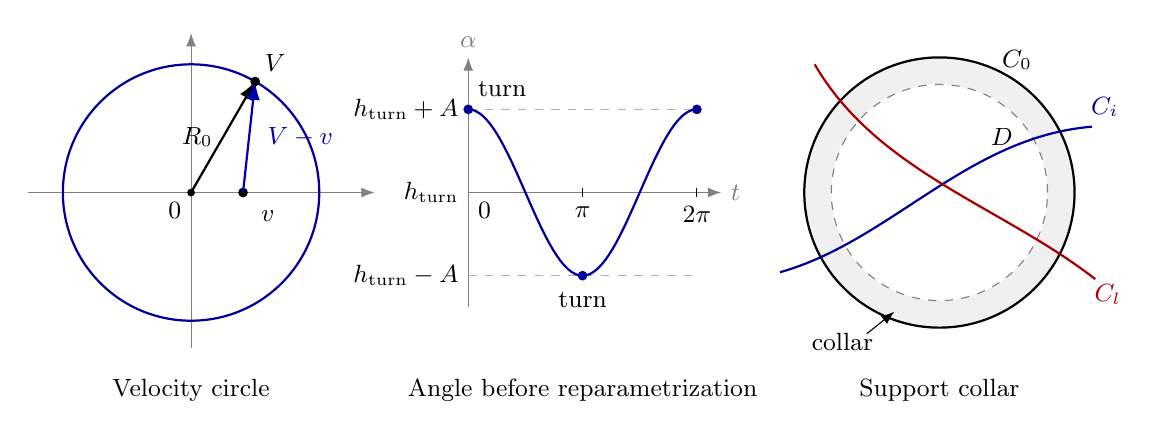
\begin{tikzpicture}[scale=.88,>=Latex,font=\small]
 \begin{scope}
  \draw[->,gray] (-2.35,0)--(2.65,0);
  \draw[->,gray] (0,-2.25)--(0,2.3);
  \draw[thick,blue!60!black] (0,0) circle (1.85);
  \fill (0,0) circle (1.6pt) node[below left] {$0$};
  \fill (.75,0) circle (2pt) node[below right=3pt] {$v$};
  \coordinate (V) at (60:1.85);
  \draw[->,thick] (0,0)--(V) node[midway,left] {$R_0$};
  \draw[->,thick,blue!70!black] (.75,0)--(V)
    node[midway,right=3pt] {$V-v$};
  \fill (V) circle (2pt) node[above right] {$V$};
  \node at (0,-2.85) {Velocity circle};
 \end{scope}
 \begin{scope}[xshift=4cm]
  \draw[->,gray] (0,-1.65)--(0,1.95) node[above] {$\alpha$};
  \draw[->,gray] (0,0)--(3.65,0) node[right] {$t$};
  \draw[dashed,gray!60] (0,1.2)--(3.3,1.2);
  \draw[dashed,gray!60] (0,-1.2)--(3.3,-1.2);
  \node[left] at (0,1.2) {$h_{\mathrm{turn}}+A$};
  \node[left] at (0,0) {$h_{\mathrm{turn}}$};
  \node[left] at (0,-1.2) {$h_{\mathrm{turn}}-A$};
  \draw[thick,blue!60!black,domain=0:360,samples=81]
    plot ({3.3*\x/360},{1.2*cos(\x)});
  \fill[blue!60!black] (0,1.2) circle (2pt);
  \fill[blue!60!black] (1.65,-1.2) circle (2pt);
  \fill[blue!60!black] (3.3,1.2) circle (2pt);
  \node[above right] at (0,1.25) {turn};
  \node[below] at (1.65,-1.3) {turn};
  \node[below right] at (0,0) {$0$};
  \draw (1.65,.06)--(1.65,-.06) node[below] {$\pi$};
  \draw (3.3,.06)--(3.3,-.06) node[below] {$2\pi$};
  \node at (1.65,-2.85) {Angle before reparametrization};
 \end{scope}
 \begin{scope}[xshift=10.8cm]
  \fill[gray!12] (0,0) circle (1.95);
  \fill[white] (0,0) circle (1.56);
  \draw[thick] (0,0) circle (1.95);
  \draw[dashed,gray] (0,0) circle (1.56);
  \draw[thick,blue!60!black] (-2.3,-1.15) .. controls (-.7,-.7) and (.4,.8) .. (2.2,.95);
  \draw[thick,red!65!black] (-1.8,1.85) .. controls (-.9,.3) and (.9,-.2) .. (2.25,-1.25);
  \node[blue!60!black,above right] at (2.05,.95) {$C_i$};
  \node[red!65!black,below right] at (2.1,-1.18) {$C_l$};
  \node[above] at (1.12,1.63) {$C_0$};
  \node at (-1.4,-2.15) {collar};
  \draw[->,thin] (-1.05,-2.04)--(-.65,-1.72);
  \node at (.9,.8) {$D$};
  \node at (0,-2.85) {Support collar};
 \end{scope}
\end{tikzpicture}
\caption{Velocity circle, its angular parametrization, and the support collar.
The circle in $P=\operatorname{span}(Y,C)^\perp$ has radius
$R_0=(|v|^2+a^2)^{1/2}$; $V-v$ is the correction vector.
The middle panel plots $\alpha=h_{\mathrm{turn}}+A\cos t$ before the
positive reparametrization that gives mean velocity $v$.
It has two turns per period, at $t=0\equiv2\pi$ and $t=\pi$.
There $\alpha_y=(h_{\mathrm{turn}})_y\pm A_y$, even after
reparametrization, so a large transverse derivative can control both turns.
The angle graph also applies when $A>\pi$ and the velocity path wraps
around the circle.  As $a$ vanishes at $C_0$, the path contracts smoothly
to $v$, while the circle retains radius $|v|>0$.
The exact immersions approach the old map in $C^2$ outside $D$
as the fast scale tends to zero.}
\label{fig:velocity-collar}
\end{figure}


\subsection{A small function with a prescribed transverse derivative}

We will need a large value of $(h_{\mathrm{turn}})_y$ along the later
curves away from the boundary, while keeping $h_{\mathrm{turn}}$ small
in value.  The finite-tangency hypothesis of
Proposition~\ref{prop:primitive-addition} gives exactly this freedom.

\begin{lemma}
\label{lem:small-value-derivative}
Let $K$ be a compact subset of a finite union of smooth embedded curves
in the interior of a coordinate disk.  Suppose the curves have only
finitely many intersections and only finitely many tangencies to
$\partial_y$ near $K$, with no shared curve arcs.  Given $B>0$ and
$\epsilon>0$, there is $h\in C_c^\infty(D)$ such that
\[
 \|h\|_{C^0}<\epsilon,\qquad h_y=B\quad\text{on }K.
\]
The support may be kept in any fixed precompact open neighborhood of $K$.
\end{lemma}

\begin{proof}
Place the finitely many intersections and vertical tangencies in
pairwise disjoint small disks centered at points $p$.  Choose bumps
$\chi_p$ equal to one on smaller disks and supported in the larger ones.
The function
\[
 h^{\mathrm{pre}}=\sum_p\chi_p B(y-y(p))
\]
has arbitrarily small sup norm when the disks are sufficiently small,
and $(h^{\mathrm{pre}})_y=B$ on the smaller disks.
Choose still smaller cores.  Outside those cores, the relevant compact
curve set is covered by finitely many patches containing just one
curve.  In such a patch choose a defining function $f_j$ with
$(f_j)_y\ne0$; the latter condition expresses transversality to
$\partial_y$.  Choose smooth patch cutoffs $\chi_j$ whose sum is one
on the part of $K$ where $(h^{\mathrm{pre}})_y\ne B$.
Add the functions
\[
 h_j=\chi_j f_j
       \frac{B-(h^{\mathrm{pre}})_y}{(f_j)_y}
       \eta_j(f_j/\delta_j),
\]
where $\eta_j$ is one near zero and has compact support.
On the curve $f_j=0$, differentiation gives exactly
\[
 (h_j)_y=\chi_j\bigl(B-(h^{\mathrm{pre}})_y\bigr).
\]
All derivatives of the cutoffs in this identity have a factor $f_j$
and therefore vanish there.  Thus
$h=h^{\mathrm{pre}}+\sum_jh_j$ has $h_y=B$ on $K$, including the
transition annuli of the special-point bumps.  Each quotient is bounded
on its fixed patch, so taking the finitely many $\delta_j$ sufficiently
small makes the additional sup norms as small as desired.  The supports
stay within the prescribed neighborhood.
\end{proof}

\subsection{Uniform normal bounds and the choice at turns}

For the rest of this section evaluate the slow data at $G=F$.
Let $S_0$ be the length of the projection of $C$ to
$\operatorname{span}(X,Y)^\perp$, and let $n_0^*$ be its unit direction.
This projection never vanishes: if $C$ belonged to
$\operatorname{span}(X,Y)$, applying $P$ would force its $X$ coefficient
to be zero since $PX=V\ne0$, contradicting independence of $C,Y$.
Compactness gives positive lower and upper bounds for $S_0$, uniformly
over all angular values.  A complementary unit normal is
\[
 m_0^*=-\sin\alpha\,e_1+\cos\alpha\,e_2.
\]
It is perpendicular to $X,Y,C$, and hence also to $n_0^*$.  Set
\begin{equation}
 D_0^*=\langle X_y,n_0^*\rangle,
 \qquad N_0^*=\langle X_y,m_0^*\rangle.
 \label{eq:limiting-mixed-components}
\end{equation}
The derivative here holds the periodic parameter fixed.  Directly,
\[
 X_y=(F_x-v)_y+(R_0)_yp+
 R_0\bigl(\cos\alpha(e_1)_y+\sin\alpha(e_2)_y
                    +\alpha_y m_0^*\bigr).
\]
The term containing $\alpha_y$ drops out of $D_0^*$, so
\begin{equation}
 |D_0^*|\le C_0,
 \qquad N_0^*=R_0\alpha_y+E_0,\quad |E_0|\le C_0,
 \label{eq:derivative-independent-bounds}
\end{equation}
where $C_0$ is independent of $h_{\mathrm{turn}}$, its derivatives,
and the reparametrization.  These estimates hold over all angular
values.  The same independence holds for the bounds on $S_0$ and
$1/S_0$.

Write
\[
 k_+=K_{\gamma_+}\det(\gamma_+)
\]
with determinant in $(x,y)$ coordinates, and write
$Y_i=b_i\partial_x+c_i\partial_y$ on the disk.  At a crossing
$C_i\cap C_0$, the loop is constant and $X=F_x$.  Since $a$ is flat,
the prescribed metric $\gamma_+$ has the old curvature there.
Consequently the strict condition $Q_{0i}(F)>0$ is exactly
\begin{equation}
 (D_0^*b_i+S_0c_i)^2+k_+b_i^2>0.
 \label{eq:collar-inequality}
\end{equation}
It remains valid on the later curves in a sufficiently thin collar for
all path angles.  Indeed $A_{\mathrm{sm}}$ tends to zero at the boundary,
and $D_0^*$ contains no angular derivative.  Compactness confines the
later curve portions of a thin collar to neighborhoods of their
finitely many crossings with $C_0$.  The collar can also avoid every
later mutual crossing, because there are no triple intersections.
The same inequality holds if the path angles are translated by any
sufficiently small value of $h_{\mathrm{turn}}$.  Thus this collar
estimate remains available even if the eventual interior support
neighborhood of $h_{\mathrm{turn}}$ overlaps its inner part.

Let $K$ be the compact union of the later curve portions in the disk
outside this collar.  By Lemma~\ref{lem:small-value-derivative},
we may prescribe $(h_{\mathrm{turn}})_y=B_*$ on $K$ with arbitrarily
small values of $h_{\mathrm{turn}}$.  The support can lie in a fixed compact neighborhood of $K$ inside $D$,
while a smaller boundary collar remains unchanged.  On any overlap
with the collar estimate, smallness in value preserves that estimate.
For any fixed threshold $T$, choose
\begin{equation}
 B_* > \|A_y\|_{C^0}
        +\frac{T+C_0+1}{\min R_0}.
 \label{eq:turn-size-choice}
\end{equation}
Equations \eqref{eq:turn-derivative} and
\eqref{eq:derivative-independent-bounds} then give
$N_0^*>T+1$ at both turns on $K$.  After making the values of
$h_{\mathrm{turn}}$ small enough to retain convex-hull membership,
choose the positive density as above.  That reparametrization does not
change the turn derivative identity.

We summarize the construction in the form needed by the next section.

\begin{lemma}[Velocity loop]
\label{lem:velocity-loop}
Under the hypotheses of Proposition~\ref{prop:primitive-addition}, fix
any finite threshold $T$.  There is a neighborhood of the 2-jet section
of $F$ over $\overline D$ and a small exterior neighborhood, on which
one can choose smooth $2\pi$-periodic vectors $V,w$ as in
\eqref{eq:velocity-plane}--\eqref{eq:leading-velocity}, with
\[
 |V|=R_0>0,\qquad \avg V=v,\qquad \avg w=0.
\]
They depend smoothly on position and the 2-jet; $w$ extends smoothly by
zero outside $D$.  The leading derivatives $(X,Y)$ have metric
$\gamma(G)+a^2dx^2$.  At $G=F$, the limiting normal data defined in
\eqref{eq:limiting-mixed-components} have uniform bounds
\eqref{eq:derivative-independent-bounds}, a positive lower bound for
$S_0$, and the collar inequality \eqref{eq:collar-inequality}.
On the remaining compact portions of the later curves, the only zeros
of $\alpha_\theta$ are the two turns, and there $|N_0^*|>T$.
The bounds for $S_0,1/S_0,D_0^*$ and the error $E_0$ can be fixed before
choosing $T$ and $B_*$.
\end{lemma}

All choices in this section are now fixed before the fast oscillation
scale is sent to zero.  In particular their higher derivatives may be
large but are finite.  The next section will use this fixed smooth
loop to produce exact immersions.  We will choose $T$ from explicit
crossing bounds in Section~\ref{sec:geometry-preservation}; those bounds
use only the quantities just shown to be independent of $T$.

\section{Realizing the primitive metric addition}
\label{sec:primitive-realization}

The velocity loop gives the desired metric at leading order.  We now remove
its oscillating errors to arbitrarily high finite order, correct the remaining
mean error by small increments, and apply
Proposition~\ref{prop:exact-correction}.  The resulting exact immersions retain
the first and second derivatives needed to control the later boundary curves.

\begin{proposition}[Realization of a velocity loop]
\label{prop:primitive-realization}
Let $M$ be a closed smooth surface and let $F:M\to\R^4$ be a smooth immersion
whose second fundamental form is nonzero at every point.  Let $D$ be a disk
with coordinates $x,y$ on a neighborhood of its closure, and let $a$ be a
smooth nonnegative function, positive on $D$ and zero on its exterior.
Suppose the following data are defined smoothly on a neighborhood of the
$2$-jets of $F$ over $\overline D$ and a collar.  For a map $G$ with jets in
that neighborhood, set
\[
 Y=G_y,\qquad C=G_{yy},\qquad
 P=\operatorname{span}(Y,C)^\perp,\qquad
 v=PG_x,\qquad R_0=(|v|^2+a^2)^{1/2}.
\]
Assume that $Y,C$ are independent and $R_0>0$.  Suppose there is a smooth
$2\pi$-periodic vector $V=V(G;\theta)$, depending only on position and the
$2$-jet of $G$, such that
\[
 V\in P,\qquad |V|=R_0,\qquad \avg_\theta V=v.
\]
Assume also that $V-v$ extends smoothly by zero across the boundary of $D$.
These hypotheses hold for the loop of Lemma~\ref{lem:velocity-loop}.

Put $h_*=\gamma(F)+a^2dx^2$, extending the added tensor by zero.  For all
sufficiently small $z>0$ there is a smooth immersion
$\widetilde f_z:M\to\R^4$ with $\gamma(\widetilde f_z)=h_*$.  To state its
derivatives, evaluate the preceding quantities at $G=F$ and write
$X=F_x-v+V$.  Uniformly on $\overline D$, with periodic arguments evaluated
at $\theta=x/z$,
\begin{equation}
\begin{aligned}
 (\widetilde f_z)_x&=X+o(1),&
 (\widetilde f_z)_y&=Y+o(1),\\
 (\widetilde f_z)_{yy}&=C+o(1),&
 (\widetilde f_z)_{xy}&=X_y+o(1),\\
 z(\widetilde f_z)_{xx}&=V_\theta+o(1).
\end{aligned}
\label{eq:realization-asymptotics}
\end{equation}
Here $X_y$ means differentiation with $\theta$ held fixed.  On the exterior
of $D$, $\widetilde f_z$ converges to $F$ in $C^2$.  There is a constant
$c>0$, independent of sufficiently small $z$, such that
\[
 \min_{p\in M}\max_{|u|=1}
       |B_{\widetilde f_z}(u,u)|\ge c,
\]
where the unit vectors use the fixed background tangent norm.
\end{proposition}

All compact neighborhoods of jets used below are chosen inside the open
sets in this statement.  Thus the stated nondegeneracies have positive
uniform margins.  Derivatives of periodic coefficients in $x,y$ will always
hold $\theta$ fixed.  We write $b_z=o_s(c_z)$ when
$|b_z|_{k,s}/c_z\to0$ for every fixed weighted differentiation order $k$.

\subsection{Removing the oscillating coefficients}

Finite-order asymptotic isometric constructions also occur in Poznyak's
planar immersion problem in $\R^3$ \cite[\S2.3, Theorem~5]{Poznyak1973}.
For the present velocity loop, we give the periodic correctors and their
support properties by an explicit recursion.

For a periodic scalar or vector $b$, define
\[
 \avg b=\frac1{2\pi}\int_0^{2\pi}b(\theta)\,d\theta,
 \qquad \Pi b=b-\avg b.
\]
For $\avg b=0$, let $\mathcal I b$ be its unique periodic primitive with
mean zero.  These operations commute with differentiation in the slow
variables $x,y$.

\begin{lemma}[Finite periodic expansion]
\label{lem:finite-periodic-expansion}
Under the hypotheses of Proposition~\ref{prop:primitive-realization}, for
each integer $L\ge2$ there are periodic differential operators
$U_1,\ldots,U_L$ with values in $\R^4$, and symmetric tensor differential
operators $E_1,\ldots,E_{L-1}$, for which
\begin{equation}
 f_z[G]=G+\sum_{j=1}^L z^jU_j(G;x/z)
 \label{eq:finite-ansatz}
\end{equation}
has the exact expansion
\begin{equation}
 \gamma(f_z[G])
   =a^2dx^2+\mathcal P_z(G)
        +\sum_{r=L}^{2L}z^r\mathcal R_r(G;x/z),
 \qquad
 \mathcal P_z(G)=\gamma(G)+\sum_{r=1}^{L-1}z^rE_r(G).
 \label{eq:finite-metric-expansion}
\end{equation}
Each $U_j$ has mean zero.  The operators $U_j,E_r,\mathcal R_r$ are smooth,
supported on $\overline D$, and polynomial in jets above order two, with
smooth coefficients in the $2$-jet and position, and, where appropriate,
$\theta$.  One may take the differential orders of $U_j$ and $E_r$ to be at
most $2j$ and $2r+2$, respectively.
\end{lemma}

\begin{proof}
Put $w=V-v$ and $X=G_x+w$, and take $U_1=\mathcal Iw$.  Orthogonal
decomposition into $P$ and $P^\perp$ gives
\[
 |X|^2=|G_x-v|^2+R_0^2=|G_x|^2+a^2,
 \qquad X\cdot Y=G_x\cdot G_y.
\]
Thus $X,Y$ induce exactly the leading metric
$\gamma(G)+a^2dx^2$.  Moreover $Y\cdot U_1=C\cdot U_1=0$, so
\begin{equation}
 Y\cdot U_{1,y}=(Y\cdot U_1)_y-C\cdot U_1=0.
 \label{eq:first-yy-cancellation}
\end{equation}
This cancels the $yy$ coefficient at order $z$ before any higher corrector
is introduced.

We construct $U_{r+1}$ from $U_1,\ldots,U_r$.  In the formal first
derivatives of \eqref{eq:finite-ansatz}, write
\[
 f_x=X+\sum_{i\ge1}z^i\mathsf A_i,
 \qquad f_y=Y+\sum_{i\ge1}z^i\mathsf B_i,
 \qquad
 \mathsf A_i=U_{i,x}+U_{i+1,\theta},\quad
 \mathsf B_i=U_{i,y}.
\]
Absent terms are set to zero; in particular $\mathsf A_L=U_{L,x}$.
At step $r$, all $\mathsf A_i$ with $i<r$ and all $\mathsf B_i$ with
$i\le r$ are already known.  The new $U=U_{r+1}$ occurs in the $xx,xy$
coefficients at order $z^r$, and in the $yy$ coefficient at order
$z^{r+1}$.  Removing their fluctuations requires
\begin{equation}
 Y\cdot U_\theta=h,\qquad
 Y\cdot U_y=j,\qquad
 \Pi(X\cdot U_\theta)=e,
 \label{eq:periodic-corrector-system}
\end{equation}
where
\begin{align}
 h&=-\Pi\left(X\cdot\mathsf B_r+Y\cdot U_{r,x}
             +\sum_{i=1}^{r-1}\mathsf A_i\cdot\mathsf B_{r-i}\right),
       \label{eq:periodic-rhs-h}\\
 e&=-\Pi\left(X\cdot U_{r,x}
             +\frac12\sum_{i=1}^{r-1}
                        \mathsf A_i\cdot\mathsf A_{r-i}\right),
       \label{eq:periodic-rhs-e}\\
 j&=-\frac12\Pi\sum_{i=1}^{r}
                         \mathsf B_i\cdot\mathsf B_{r+1-i}.
       \label{eq:periodic-rhs-j}
\end{align}
For example, at $r=1$ these are
\[
 h=-\Pi(X\cdot U_{1,y}+Y\cdot U_{1,x}),\qquad
 e=-\Pi(X\cdot U_{1,x}),\qquad
 j=-\tfrac12\Pi|U_{1,y}|^2.
\]
Thus the first correction removes the $xx,xy$ fluctuations at order $z$
and the $yy$ fluctuation at order $z^2$.  Every right side has mean zero.
This is precisely the compatibility required by the first two equations
of \eqref{eq:periodic-corrector-system} when $\avg U=0$.

Set $H=\mathcal I h$.  There is a unique
$T\in\operatorname{span}(Y,C)$ satisfying
\begin{equation}
 Y\cdot T=H,\qquad C\cdot T=H_y-j.
 \label{eq:corrector-span-part}
\end{equation}
It is obtained by inverting the Gram matrix of $Y,C$, and has mean zero.
Since $Y_y=C$, these equations imply
\[
 Y\cdot T_\theta=h,\qquad Y\cdot T_y=j.
\]
If $Z\in P$, then $Y\cdot Z=C\cdot Z=0$ and hence
$Y\cdot Z_y=0$.  The remaining part of $U$ can therefore be written
$Z=\mathcal I W$, where $W\in P$ has mean zero and must solve
\begin{equation}
 \Pi(V\cdot W)=r_0,
 \qquad r_0=e-\Pi(X\cdot T_\theta).
 \label{eq:covariance-equation}
\end{equation}

Here is an explicit solution which remains regular at $a=0$.  Regard the
following matrices as operators on the Euclidean plane $P$:
\[
 \Sigma=\avg\bigl((V-v)\otimes(V-v)\bigr),
 \qquad \mathsf M=\Id_P-\frac{\Sigma}{R_0^2}.
\]
For a unit vector $q\in P$,
\begin{equation}
 R_0^2\langle\mathsf Mq,q\rangle
   =\avg\bigl(R_0^2-(q\cdot V)^2\bigr)+(q\cdot v)^2.
 \label{eq:covariance-positive}
\end{equation}
Both terms are nonnegative.  Equality would force $V$ to take values only
in $\{R_0q,-R_0q\}$.  Continuity on the period circle would make $V$
constant, contrary to the additional equality $q\cdot v=0$.
Consequently $\mathsf M$ is positive definite.  Its inverse is smooth and
uniformly bounded on the compact family under consideration.  At $a=0$,
the loop is constant, $V=v$, and $\mathsf M=\Id_P$.

Define
\begin{equation}
 \begin{aligned}
 m&=\mathsf M^{-1}\avg(Vr_0),\\
 h_1&=r_0+\frac{(V-v)\cdot m}{R_0^2},\\
 W&=\frac{Vh_1-m}{R_0^2}.
 \end{aligned}
 \label{eq:covariance-solve}
\end{equation}
Then $\avg h_1=0$ and
\[
 \avg(Vh_1)=\avg(Vr_0)+\frac{\Sigma m}{R_0^2}=m.
\]
Hence $\avg W=0$, and $|V|^2=R_0^2$ gives
\[
 \Pi(V\cdot W)=h_1-\frac{(V-v)\cdot m}{R_0^2}=r_0.
\]
Thus $U_{r+1}=T+\mathcal I W$ solves
\eqref{eq:periodic-corrector-system} with mean zero.

This construction is triangular: it changes no previously fixed lower
coefficient.  Induction through $r=L-1$, together with
\eqref{eq:first-yy-cancellation}, makes every metric coefficient of orders
$1,\ldots,L-1$ independent of $\theta$.  Define $E_r$ to be that
coefficient.  The remaining finite coefficients give
$\mathcal R_L,\ldots,\mathcal R_{2L}$ in
\eqref{eq:finite-metric-expansion}.

It remains to check the regularity properties needed for the next stage.
The initial coefficient $U_1$ is a smooth function of the $2$-jet.
Differentiation preserves the class of polynomials in higher jets with
smooth low-jet coefficients, as do multiplication, averaging and
$\mathcal I$.  The Gram and covariance inverses depend only on the
$2$-jet.  Equations \eqref{eq:periodic-rhs-h}--\eqref{eq:covariance-solve}
therefore preserve this class.  If $U_i$ has order at most $2i$ for
$i\le r$, the right side $h$ has order at most $2r+1$; the derivative
$H_y$ raises this by at most one.  All other terms have order at most
$2r+2$.  This proves the asserted order of $U_{r+1}$, and the same
coefficient formulas give order at most $2r+2$ for $E_r$.

Finally, $w$ is smoothly zero on the exterior, so $U_1$ is as well.  If
the previous correctors vanish there, all right sides in
\eqref{eq:periodic-rhs-h}--\eqref{eq:periodic-rhs-j} vanish there and the
linear construction gives $U_{r+1}=0$.  The formulas are smooth on the
collar, including its boundary, so this is smooth extension by zero to
every order.  The same reasoning applies to $E_r$ and $\mathcal R_r$.
\end{proof}

\subsection{Correcting the mean and selecting the scales}

The preceding lemma leaves two errors: a finite mean operator
$\mathcal P_z-\gamma$, and a remainder beginning at $z^L$.  We first record
how the latter behaves when the slow map depends on $z$.
Suppose
\begin{equation}
 G\longrightarrow F\text{ in }C^3,
 \qquad j^2G=O_s(1),\qquad s=z^\sigma,
 \qquad 0<\sigma<1.
 \label{eq:slow-map-bounds}
\end{equation}
A jet of order $k>2$ is $O_s(s^{2-k})$.  Since the expansion has finitely
many coefficients, Lemma~\ref{lem:finite-periodic-expansion} supplies an
integer $p_1\ge0$ such that they and their required periodic derivatives
are all $O_s(s^{-p_1})$.  This exponent is independent of the weighted
differentiation order; the constants may depend on that order.  Indeed
each higher-jet monomial loses the sum of the quantities $k-2$ for its
factors, while weighted differentiation of its coefficients loses no
additional power of $s$.

Substitution of $\theta=x/z$ changes these estimates to $O_z(s^{-p_1})$:
a derivative in $\theta$ costs $z^{-1}$, and a slow derivative costs
$s^{-1}\le z^{-1}$.  In particular,
\begin{equation}
 \gamma(f_z[G])-a^2dx^2-\mathcal P_z(G)
       =O_z(z^Ls^{-p_1}).
 \label{eq:fast-remainder-bound}
\end{equation}

For later use, differentiating the finite ansatz gives
\begin{align*}
 f_x&=X+\sum_{j=1}^L z^jU_{j,x}
           +\sum_{j=2}^L z^{j-1}U_{j,\theta},\\
 f_y&=Y+\sum_{j=1}^L z^jU_{j,y},
 &f_{yy}&=C+\sum_{j=1}^L z^jU_{j,yy},\\
 f_{xy}&=X_y+\sum_{j=1}^L z^jU_{j,xy}
           +\sum_{j=2}^L z^{j-1}U_{j,\theta y},\\
 zf_{xx}&=V_\theta+zG_{xx}
       +\sum_{j=1}^L z^{j+1}U_{j,xx}
       +2\sum_{j=1}^L z^jU_{j,x\theta}
       +\sum_{j=2}^L z^{j-1}U_{j,\theta\theta}.
\end{align*}
All coefficients on these right sides are evaluated at $G$ and
$\theta=x/z$.  Each error contains a positive power of $z$ and at most
two further slow derivatives.  Thus
\begin{equation}
 \sigma(p_1+2)<1
 \label{eq:fast-asymptotic-scale}
\end{equation}
makes these errors uniformly small.  The leading terms converge uniformly
to their values at $F$, including $X_y$, because of the $C^3$ convergence
in \eqref{eq:slow-map-bounds}.  The same estimates show
$\|f_z[G]\|_{C^k}=O(z^{-k})$ for each fixed $k$.

We now construct a slow map satisfying \eqref{eq:slow-map-bounds} for
which the mean error is small enough for exact correction.

\begin{proof}[Proof of Proposition~\ref{prop:primitive-realization}]
Choose the integers $R,N$ in Proposition~\ref{prop:exact-correction} for
the fixed positive metric $h_*$.  Fix an integer
\[
 L>N+R+1
\]
and construct the operators in Lemma~\ref{lem:finite-periodic-expansion}.
Obtain $p_1$ as above and let $p$ be the exponent in
Proposition~\ref{prop:small-increment} for $\mathcal P_z$, with its
perturbation parameter equal to $z$.  These exponents may depend on $L$.
The exponent $p$ is independent of the accuracy parameter in that
proposition.

Define
\[
 d_1=\tfrac14,\qquad d_{l+1}=\tfrac65d_l,
\]
and choose a finite $m\ge2$ with $2d_m>N+R+1$.  Next choose
$\sigma>0$ so small that
\begin{equation}
 \sigma<1,\qquad \sigma(p_1+2)<1,\qquad
 \sigma p<\tfrac12,\qquad \sigma<\tfrac14d_1,
 \qquad L-R-\sigma p_1>N.
 \label{eq:slow-scale-choice}
\end{equation}
Set
\[
 \sigma_l=\frac{l\sigma}{m-1}\quad(0\le l\le m-1),\qquad
 s_l=z^{\sigma_{l-1}},\qquad \delta_l=z^{d_l}
       \quad(1\le l\le m).
\]
Thus $s_1=1$ and $s_m=z^\sigma$.  Fix phase data for $F$ from
Lemma~\ref{lem:phase-data}, with reference tensor $h_0=\gamma(F)$.

Start with
\[
 G_1=(1-\delta_1^2)^{1/2}F,
 \qquad
 H_l=\delta_l^{-2}\bigl(\gamma(F)-\mathcal P_z(G_l)\bigr).
\]
The family $G_1$ is uniformly smooth and $\mathcal P_z-\gamma$ begins
with $z$, whereas $\delta_1^2=z^{1/2}$.  Hence $H_1\to h_0$ in every
smooth norm.  We inductively construct $G_l$ so that
\begin{equation}
 j^2G_l,H_l=O_{s_l}(1),\qquad
 G_l\to F\text{ in }C^3,\qquad H_l\to h_0\text{ in }C^0.
 \label{eq:slow-induction}
\end{equation}

For $l<m$, apply Proposition~\ref{prop:small-increment} at $G_l$ with
amplitude $\delta_l$, scales $s_l$ and $\tau=s_{l+1}$, and input tensor
\[
 H_l-(\delta_{l+1}/\delta_l)^2h_0.
\]
This tensor lies in the allowed neighborhood for small $z$.  If
\[
 \kappa=\min\left\{\frac{\sigma}{m-1},\frac12\right\}>0,
\]
the smallness parameter of that proposition satisfies
\[
 \eta=\frac{s_{l+1}}{s_l}+zs_{l+1}^{-p}=O(z^\kappa).
\]
Only now choose its finite accuracy $q_l$ so large that
\[
 d_l+\kappa q_l>2d_{l+1}.
\]
The other error exponent is positive as well:
\[
 3d_l-\sigma_l-2d_{l+1}
      =\tfrac35d_l-\sigma_l>0.
\]
Thus the increment $U$ supplied by that proposition gives
\[
 \mathcal P_z(G_l+U)
      =\gamma(F)-\delta_{l+1}^2h_0
                       +o_{s_{l+1}}(\delta_{l+1}^2).
\]
Set $G_{l+1}=G_l+U$.  Then $H_{l+1}=h_0+o_{s_{l+1}}(1)$.
Furthermore
\[
 |j^2U|_{k,s_{l+1}}\le C_k z^{d_l-\sigma_l}\longrightarrow0,
 \qquad
 \|U\|_{C^3}\le C z^{d_l-2\sigma_l}\longrightarrow0.
\]
Bounds on the old terms improve when the weighted scale decreases, so
\eqref{eq:slow-induction} is preserved.  All choices are finite.  The
choice of $q_l$ affects only the eventual threshold on $z$; it does not
change $p$ or the already fixed scales.

Take $G=G_m$ and $s=s_m$.  The construction gives
\[
 \mathcal P_z(G)-\gamma(F)=O_s(z^{2d_m}).
\]
With $f_z=f_z[G]$, equation~\eqref{eq:fast-remainder-bound} now yields
\begin{equation}
 \|\gamma(f_z)-h_*\|_{C^R}
   \le C\bigl(z^{2d_m-\sigma R}
                    +z^{L-R-\sigma p_1}\bigr)=O(z^N).
 \label{eq:realization-metric-error}
\end{equation}
The first exponent exceeds $N$ because $2d_m>N+R+1$ and $\sigma<1$;
the second was imposed in \eqref{eq:slow-scale-choice}.  We also have
$\|f_z\|_{C^k}=O(z^{-k})$ through $k=R+2$, and the displayed derivative
formulas prove \eqref{eq:realization-asymptotics} for $f_z$ before exact
correction.  On the exterior $f_z=G$, so $f_z\to F$ in $C^3$ there.
Moreover, \eqref{eq:realization-metric-error} and positivity of $h_*$
guarantee that $f_z$ is immersive for small $z$.

To check the remaining hypothesis of
Proposition~\ref{prop:exact-correction}, project $C=F_{yy}$ to the
orthogonal complement of $\operatorname{span}(X,Y)$.  This projection
never vanishes: if $C=bX+cY$, projection to $P$ gives $0=bV$, hence
$b=0$, contrary to the independence of $C,Y$.  Its length consequently
has a positive minimum on the compact position--phase set.  The
convergence of $(f_z)_x,(f_z)_y,(f_z)_{yy}$ implies a uniform positive
lower bound for $|B_{f_z}(\partial_y,\partial_y)|$ on $\overline D$.
The fixed upper bound on the background length of $\partial_y$ converts
this to the unit-vector bound.  On the exterior the same bound follows
from $C^2$ convergence to $F$ and the nonvanishing of $B_F$.

Proposition~\ref{prop:exact-correction} therefore gives smooth
$\widetilde f_z$ inducing $h_*$ with
$\|\widetilde f_z-f_z\|_{C^2}=o(1)$.  This preserves all the derivative
asymptotics, including the scaled $xx$ derivative, and gives the stated
exterior $C^2$ convergence.  The same argument using the $yy$ component
on the disk, and convergence to $F$ on the exterior, gives the positive
second-form lower bound for $\widetilde f_z$.
\end{proof}

The primitive metric is now realized exactly.  The next section uses the
unscaled $yy$ and $xy$ limits together with the exact Gauss equation to
determine the component of $B_{xx}$ along $B_{yy}$.  The scaled $xx$ limit
controls the complementary normal component.  These are precisely the
second-form data needed to preserve the normal and crossing conditions
for the remaining disks.

\section{Preserving the later boundary conditions}
\label{sec:geometry-preservation}

We complete Proposition~\ref{prop:primitive-addition}.  The analytic
construction in Proposition~\ref{prop:primitive-realization} supplies
exact immersions for $\gamma_+$ with the leading derivatives of the
chosen loop.  We must show that their second forms preserve the later
curve conditions and that their preferred normals extend globally.
The crossing calculation below also specifies a turn threshold using
only the bounds that were fixed before the loop's large derivative.

\subsection{The exact second form}

Choose the loop of Lemma~\ref{lem:velocity-loop}, with the turn threshold
to be specified below, and let $\widetilde f_z$ be the resulting exact
immersions from Proposition~\ref{prop:primitive-realization}.  On the
disk their $yy$ second form has the representation
\[
 B_{\widetilde f_z}(\partial_y,\partial_y)=S n^*,\qquad
 |n^*|=1,\qquad S>0,
\]
for all sufficiently small $z$.  Indeed its limiting value is
$S_0n_0^*$ and $S_0$ has a positive minimum.  Project $m_0^*$ to the line
in the new normal plane perpendicular to $n^*$ and normalize; the
resulting $m^*$ is well defined and close to $m_0^*$.
Write
\[
 B_{\widetilde f_z}(\partial_x,\partial_y)=D^* n^*+N^* m^*,\qquad
 k=K_{\gamma_+}\det(\gamma_+).
\]
The determinant is in the $(x,y)$ coordinates.  The Gauss equation gives
\begin{equation}
 B_{yy}=(S,0),\qquad B_{xy}=(D^*,N^*),\qquad
 B_{xx}=\left(\frac{k+(D^*)^2+(N^*)^2}{S},\,L^*\right)
 \label{eq:exact-second-form}
\end{equation}
in the orthonormal frame $(n^*,m^*)$.  We have used
$\langle B_{xx},B_{yy}\rangle-|B_{xy}|^2=k$.
Thus the exact metric determines the first component of $B_{xx}$ from
the unscaled $yy$ and $xy$ data.  Only its second component, $L^*$,
requires the scaled $xx$ asymptotic from the realization theorem.
The derivative asymptotics of the exact realization imply, uniformly
on $\overline D$,
\begin{equation}
 \begin{gathered}
 S=S_0+o(1),\qquad n^*=n_0^*+o(1),\qquad
 D^*=D_0^*+o(1),\qquad N^*=N_0^*+o(1),\\
 zL^*=R_0\alpha_\theta+o(1).
 \end{gathered}
 \label{eq:second-form-limits}
\end{equation}
The final identity follows because
$V_\theta=R_0\alpha_\theta m_0^*$ is already normal to the limiting
pair $(X,Y)$.

For later use, write $Y_i=b_i\partial_x+c_i\partial_y$.  Formula
\eqref{eq:exact-second-form} gives the exact identities
\begin{equation}
 \begin{aligned}
 S\langle B(Y_i,Y_i),n^*\rangle
    &=(D^*b_i+Sc_i)^2+(k+(N^*)^2)b_i^2,\\
 \langle B(Y_i,Y_i),m^*\rangle
    &=L^*b_i^2+2N^*b_ic_i.
 \end{aligned}
 \label{eq:pure-direction-components}
\end{equation}
These two expressions separate the two mechanisms of the construction:
a large angular velocity gives a large $L^*$, whereas at a turn a large
transverse derivative gives a large $N^*$.

\subsection{Crossing thresholds without circular choices}

At a mutual later crossing inside $D$, both $b_i,b_l$ are nonzero.
Put
\[
 u_i=\partial_x+t_i\partial_y,\qquad
 u_l=\partial_x+t_l\partial_y,
 \qquad t_i=c_i/b_i,\quad t_l=c_l/b_l.
\]
The finitely many slopes are bounded.  From
\eqref{eq:exact-second-form}, the pure and mixed vectors are
\begin{equation}
 \begin{aligned}
 P_i:=B(u_i,u_i)
   &=\left(\frac{(N^*)^2+k+(D^*+St_i)^2}{S},\ L^*+2N^*t_i\right),\\
 P_l:=B(u_l,u_l)
   &=\left(\frac{(N^*)^2+k+(D^*+St_l)^2}{S},\ L^*+2N^*t_l\right),\\
 Z_{il}:=B(u_i,u_l)
   &=\left(\frac{(N^*)^2+k+(D^*+St_i)(D^*+St_l)}{S},\
             L^*+N^*(t_i+t_l)\right).
 \end{aligned}
 \label{eq:crossing-components}
\end{equation}
In particular
\begin{equation}
 Z_{il}-P_i=(t_l-t_i)(D^*+St_i,N^*).
 \label{eq:mixed-pure-difference}
\end{equation}

Choose bounds $0<s_-\le S\le s_+$, $|D^*|\le d_+$, and $|k|\le K_0$
on the entire closed disk and over all angular values, together with a
fixed bound on the finitely many crossing slopes.  They can be chosen before
the turn derivative: the limiting bounds for $S_0,1/S_0,D_0^*$ are
independent of that derivative, and after the loop is fixed,
\eqref{eq:second-form-limits} transfers slightly enlarged bounds to the
exact immersions for sufficiently small $z$.  There are constants
$C_1,C_2$ depending only on these bounds such that
\begin{equation}
 \begin{aligned}
 \langle P_j,n^*\rangle&\ge (N^*)^2/s_+-C_1,\\
 \left\langle Z_{il},\frac{P_j}{|P_j|}\right\rangle
 &\ge (N^*)^2/s_+-C_2(1+|N^*|),\qquad j=i,l,
 \end{aligned}
 \label{eq:uniform-crossing-bound}
\end{equation}
whenever the right side of the first line is positive.  To see the
second line, use
$\langle Z_{il},\widehat P_j\rangle
\ge |P_j|-|Z_{il}-P_j|$ and
\eqref{eq:mixed-pure-difference}.  In particular these estimates do not
depend on $L^*$.

Also
\[
 K_{\gamma_+}|u_i\wedge u_l|_{\gamma_+}^2
 =k(t_i-t_l)^2.
\]
We can therefore fix a finite threshold $T$ so large that $T^2>K_0+1$
and, when $|N^*|>T$, both pure vectors have positive dot with $n^*$ and
both mixed projections in \eqref{eq:uniform-crossing-bound} exceed
\[
 \sqrt{\max\{0,-k(t_i-t_l)^2\}}+1
\]
at every crossing.  Use a margin, for example $T+2$, as the turn
threshold in Lemma~\ref{lem:velocity-loop}, and then fix the loop.
No constant used to select this threshold depends on the resulting
large value of $(h_{\mathrm{turn}})_y$.  The sufficiently small choice
of $z$ may depend on this now fixed loop.

We next show positivity of both ordered crossing invariants for all
small $z$.  If a sequence of crossing phases tends to a turn,
\eqref{eq:second-form-limits} gives $|N^*|>T$, so the preceding estimate
applies.  If its limiting phase is not a turn, then
$|L^*|\to\infty$, while $N^*$ stays bounded for the fixed loop.
All three vectors in \eqref{eq:crossing-components} have the same
leading second component $L^*$; hence
\[
 \left\langle Z_{il},\widehat P_i\right\rangle\to+\infty,
 \qquad
 \left\langle Z_{il},\widehat P_l\right\rangle\to+\infty.
\]
These two cases and compactness of the phase circle give positivity at
the finitely many crossings uniformly for small $z$.
Returning to the original directions changes each ordered invariant
by the positive factor $b_i^2b_l^2$.  Indeed pure second forms scale by
squares, so their unit directions do not change even if either $b$ is
negative.  We have proved
\begin{equation}
 Q_{il}(\widetilde f_z)>0,\qquad
 Q_{li}(\widetilde f_z)>0
 \quad\text{at all later mutual crossings in }D.
 \label{eq:preserved-crossing-q}
\end{equation}

\subsection{Avoidance along the full curves}

We now prove that on every later curve inside the disk,
$B(Y_i,Y_i)$ is nonzero and its unit direction is not $-n^*$.
Suppose otherwise along a sequence $z\downarrow0$.
At a point of failure the second component in
\eqref{eq:pure-direction-components} is zero and the first is
nonpositive, so
\begin{equation}
 (D^*b_i+Sc_i)^2+(k+(N^*)^2)b_i^2\le0,
 \qquad L^*b_i^2+2N^*b_ic_i=0.
 \label{eq:opposite-ray-failure}
\end{equation}
Take a subsequence with limiting position and periodic phase.
The limiting $b_i$ cannot be zero: the vector field $Y_i$ is nonzero,
so then $c_i\ne0$ and the first inequality would give
$S_0^2c_i^2\le0$.  Multiplying the second equality by $z$ and using
\eqref{eq:second-form-limits} now forces
$\alpha_\theta=0$ at the limiting phase.

In the boundary collar, \eqref{eq:collar-inequality} rules out the
first inequality of \eqref{eq:opposite-ray-failure}, even without its
nonnegative $(N^*)^2b_i^2$ term.  On the remaining compact curve portions,
the limiting phase must be one of the two turns and
$k+(N_0^*)^2>0$ by the threshold just chosen.  This again contradicts
the first inequality.  Therefore, for all sufficiently small $z$,
\begin{equation}
 B(Y_i,Y_i)\ne0,
 \qquad \frac{B(Y_i,Y_i)}{|B(Y_i,Y_i)|}\ne-n^*
 \quad\text{on }C_i\cap\overline D.
 \label{eq:disk-ray-avoidance}
\end{equation}
This argument needs boundedness of $N^*$ only for the fixed loop while
$z$ tends to zero.  Such a bound may depend on the chosen turn size;
it is distinct from the derivative-independent bounds used to choose
that size.

\subsection{Adjusting the normal at crossings}

It remains to give both pure vectors positive dot product with a
preferred normal at each crossing.  If their dots with $n^*$ are
already positive, no change is needed.  At each crossing, choose small
neighborhoods of the two turning phases on which $|N_0^*|>T+1$.
The uniform limits and \eqref{eq:uniform-crossing-bound} make both
dot products positive on these neighborhoods for small $z$.
Consequently any crossing requiring adjustment has phase in their
compact complement, where $|\alpha_\theta|$ has a positive lower bound.
There $|L^*|\to\infty$ uniformly, and the two pure unit vectors are
arbitrarily close to the same sign of $m^*$.
For small $z$, denote this sign by $m$ and use the path
\begin{equation}
 n_t=\frac{(1-t)n^*+t\widehat P_i}
 {|(1-t)n^*+t\widehat P_i|},\qquad 0\le t\le1.
 \label{eq:normal-crossing-path}
\end{equation}
This path is defined and avoids the opposite of either pure unit
vector.  Its numerator has nonnegative $m$ component, strictly positive
for $t>0$, whereas the opposite pure vectors have negative $m$
component.  At $t=0$, use $n^*\perp m$.
At the endpoint both required dot products are positive because
$\widehat P_i$ and $\widehat P_l$ are close.

The vectors in this construction extend smoothly to a neighborhood
of the crossing.  Strictness, together with compactness of $[0,1]$,
gives a neighborhood on which the whole path remains defined and
avoids the opposite pure directions.  Replacing $t$ by a smooth
spatial cutoff, equal to one at the crossing, makes a smooth local
normal adjustment.  Since there are no triple intersections, its
support can avoid every other curve.  The finitely many crossing
neighborhoods can be chosen pairwise disjoint and disjoint from the
boundary collar.  These changes preserve
\eqref{eq:disk-ray-avoidance}; they do not affect
\eqref{eq:preserved-crossing-q}, whose quantities are independent of
the preferred normal.

\subsection{Extension through the exterior collar}

We finish with a global preferred normal.  The exact realization
converges to $F$ in $C^2$ on the exterior of $D$.  Thus the normalized
projection of the old normal $n$ to the new normal bundle defines a
smooth unit normal $n_{\mathrm{out}}$ there for small $z$.
On a thin exterior collar, the new $yy$ second form is nonzero and
its unit direction $n^*$ is close to the old direction
$\widehat A_0$.  By \eqref{eq:boundary-invariants},
$\widehat A_0$ and $n$ are not antipodal on $C_0$.
After narrowing the collar, the normalized convex interpolation
between $n^*$ and $n_{\mathrm{out}}$ is consequently defined.
Use it to match the unchanged $n^*$ near the disk boundary to
$n_{\mathrm{out}}$ farther outside.

We check the later curves during this interpolation.  At an old
crossing $C_i\cap C_0$, the Gauss interpretation
\eqref{eq:crossing-gauss-interpretation} gives
\begin{equation}
 \langle A_0(F),A_i(F)\rangle
 =|B_F(Y_0,Y_i)|^2+
 K_\gamma|Y_0\wedge Y_i|_\gamma^2
 \ge Q_{0i}(F)>0.
 \label{eq:old-pure-crossing-dot}
\end{equation}
Thus both old endpoint normals have positive dot product with the
later pure vector: one by this inequality, and the other by
\eqref{eq:boundary-invariants}.  Continuity and exterior $C^2$
convergence retain positivity near these crossings for the new
immersion, and convex interpolation preserves it.
A sufficiently thin collar meets later curves only in these crossing
neighborhoods.  It can avoid all later mutual crossings.
Away from the disk and collar, every old strict condition persists
by exterior $C^2$ convergence and compactness.  The resulting normal
$n_+$ is global and satisfies all of
\eqref{eq:boundary-invariants} for the later indices.

The second fundamental form is nonzero on the disk because $S>0$,
and it is nonzero on the exterior by $C^2$ convergence to $F$.
Choose $z$ small enough for these properties, all the finite crossing
conditions, and the prescribed exterior error $\varepsilon$.
The exact metric is $\gamma_+$ by
Proposition~\ref{prop:primitive-realization}.  This completes the
proof of Proposition~\ref{prop:primitive-addition}.

All frame orientations in this argument were chosen inside a
coordinate disk.  The global object carried from one step to the
next is only the unit section $n_+$ of the normal bundle.  The
construction therefore applies equally to orientable and
nonorientable surfaces.

\section{Global preparation and finite assembly}
\label{sec:global-construction}

We now arrange a finite sequence of primitive additions to which
Proposition~\ref{prop:primitive-addition} applies.  The main point is the order
of the choices.  The initial immersion will be modified at the crossings of
the support boundaries, although those boundaries depend on the number of
primitive additions.  Uniform second-derivative bounds for the initial
modification allow us to choose the number of additions first.

The assertion is immediate if $M$ is empty.  The connected components
of a smooth manifold are open.  Compactness
therefore implies that $M$ has only finitely many components.  It suffices
to carry out the construction on each component: the resulting maps
together define one smooth isometric immersion on $M$.  We may thus
assume in this section that $M$ is connected.

\subsection{A spherical starting immersion}

Every closed smooth surface admits an ordinary smooth immersion into $S^3$.
Indeed, the two-dimensional case of Whitney's immersion theorem gives a
$C^1$ immersion into $\R^3$ \cite[Theorem~8, p.~274]{Whitney1944}.  Approximation in $C^1$ by a
smooth map preserves injectivity of the differential on a compact domain.
Such an approximation can be obtained by mollifying in finitely many charts
and combining the approximations with a smooth partition of unity.  Finally,
inverse stereographic projection is a diffeomorphism from $\R^3$ onto a
punctured $S^3$.  Neither step requires an orientation of the surface.

For an immersion $I:M\to S^3$, denote its second fundamental form in $S^3$
by $B_I^{S^3}$, regarded as an $\R^4$-valued tensor.  This notation avoids any
choice of unit normal to the surface in $S^3$.

\begin{lemma}[Finite-point spherical preparation]
\label{lem:spherical-preparation}
Let $M$ be a closed smooth surface and let $I:M\to S^3$ be a smooth
immersion.  There are constants $C,c>0$ and $\varepsilon_0>0$ with the
following property.  For every finite set $P\subset M$ and every
$0<\varepsilon<\varepsilon_0$, there is a smooth immersion
$I_P:M\to S^3$ such that
\[
 B_{I_P}^{S^3}(p)=0\quad(p\in P),\qquad
 \|I_P-I\|_{C^1}<\varepsilon,\qquad
 \|I_P\|_{C^2}\le C,
 \qquad I_P^*\delta_4\ge c\,g_{\mathrm{bg}},
\]
where $g_{\mathrm{bg}}$ is the fixed background metric.  The constants are
independent of the number and separation of the points of $P$.
\end{lemma}

\begin{proof}
Choose a finite atlas with precompact smaller charts covering $M$.  For each
$p\in P$, use one of these charts, translated so that $p$ has coordinates
$u=0$.  Choose radii $r_p>0$ so that the corresponding coordinate balls have
pairwise disjoint closures and lie in the larger charts.  Let $\chi$ be a
fixed smooth bump, equal to one near zero and supported in the unit ball.
In the chart at $p$, put
\[
 Q_p(u)=-\frac12\chi(u/r_p)
       \sum_{i,j=1}^2 B_I^{S^3}(\partial_i,\partial_j)(p)u_i u_j,
\]
and extend this function by zero.  Set
\[
 J=I+\sum_{p\in P}Q_p,
 \qquad I_P=\frac{J}{|J|}.
\]
For sufficiently small radii, $|J|$ stays uniformly away from zero.

At $p$, the value and first derivative of $Q_p$ vanish and
$\partial_i\partial_jQ_p=-B_I^{S^3}(\partial_i,\partial_j)(p)$.
The latter vector is tangent to $S^3$ at $I(p)$ and normal to $dI(T_pM)$.
The derivative of $v\mapsto v/|v|$ at $I(p)$ is projection to
$T_{I(p)}S^3$.  Comparing its second-derivative chain rule for $J$ and for
$I$ therefore gives
\[
 dI_P(p)=dI(p),\qquad
 \partial_i\partial_j I_P(p)
 =\partial_i\partial_j I(p)
   -B_I^{S^3}(\partial_i,\partial_j)(p).
\]
Thus the spherical normal part of the second derivative vanishes at $p$.

The $C^0,C^1,C^2$ norms of $Q_p$ are bounded respectively by
$C_0r_p^2,C_0r_p,C_0$, with $C_0$ uniform in $p$.  Since the supports are
disjoint, the corresponding norms of the sum are bounded by the maximum of
these bounds, up to the fixed atlas constants.  Normalization has uniformly
bounded derivatives on the range in question.  Taking the radii small gives
the prescribed $C^1$ closeness and a uniform $C^2$ bound.  Compactness and
the immersion property of $I$ then give the metric lower bound and preserve
immersion, after fixing $\varepsilon_0$ sufficiently small.
\end{proof}

Only the first two derivatives are controlled uniformly in this lemma.
Higher derivatives may grow when the points are close together.  The
preparation below uses only the stated bounds; constants requiring higher
derivatives will be chosen after the finite set has been fixed.

For later use, consider $F^0=\lambda I_P$, where $\lambda>0$, and write
$\gamma^0=\gamma(F^0)$.  The vector field $n^0=-I_P$ is a global unit normal
in $\R^4$.  The second fundamental forms satisfy
\begin{equation}
 B_{F^0}(v,w)
   =\lambda B_{I_P}^{S^3}(v,w)
       +\lambda^{-1}\gamma^0(v,w)n^0.
 \label{eq:spherical-radial-form}
\end{equation}
In particular, $\langle B_{F^0}(v,v),n^0\rangle>0$ for $v\ne0$.
At each point of $P$, the first term vanishes and the Gauss equation gives
$K_{\gamma^0}=\lambda^{-2}$.  For any nonzero vectors $Y_i,Y_l$ at such a
point, the quantity in~\eqref{eq:boundary-invariants} is consequently
\begin{equation}
 Q_{il}
 =\lambda^{-2}\bigl(
      \gamma^0(Y_i,Y_l)^2+|Y_i\wedge Y_l|_{\gamma^0}^2\bigr)
 =\lambda^{-2}\gamma^0(Y_i,Y_i)\gamma^0(Y_l,Y_l)>0.
 \label{eq:initial-crossing-positivity}
\end{equation}
This identity also holds when the two vectors are proportional.

\subsection{A finite list with prescribed intermediate metrics}

\begin{lemma}[Global primitive preparation]
\label{lem:global-preparation}
Let $(M,g)$ be a closed smooth Riemannian surface.  There exist a smooth
immersion $F^0:M\to\R^4$, a smooth unit normal $n^0$, and a finite list
\[
 (D_j,x_j,y_j,a_j),\qquad 1\le j\le K,
\]
with the following properties.  Each $D_j$ is a coordinate disk with smooth
boundary $C_j$; $(x_j,y_j)$ are coordinates on a neighborhood of
$\overline D_j$; and $a_j$ is smooth, positive on $D_j$, and zero on its
exterior.  Set $Y_j=\partial_{y_j}$ and
\[
 \gamma^j=\gamma(F^0)+\sum_{i=1}^j a_i^2(dx_i)^2,
 \qquad \gamma^0=\gamma(F^0).
\]
Then:
\begin{enumerate}
\item $\gamma^K=g$, and
      $\Hess_{\gamma^{j-1}}x_j(Y_j,Y_j)>0$ on $\overline D_j$.
\item The boundaries are pairwise transverse and have no triple
      intersection.  For $i\ne j$, $Y_j$ is tangent to $C_i$ at only finitely
      many points of $\overline D_j$.  At $C_i\cap C_l\cap D_j$, with
      $i,l,j$ distinct, both $dx_j(Y_i)$ and $dx_j(Y_l)$ are nonzero.
\item $B_{F^0}$ is nowhere the zero tensor, and $F^0,n^0$ satisfy all
      boundary conditions~\eqref{eq:boundary-invariants} for this list.
\end{enumerate}
\end{lemma}

\begin{proof}
Fix a spherical immersion $I$ and the uniform family of modifications in
Lemma~\ref{lem:spherical-preparation}, without yet specifying the finite set.
We make the choices below uniformly for this family.

\paragraph{Metric and cone margins.}
At any point, take a $g$-orthonormal coframe $e^1,e^2$ and the covectors
\[
 \ell_1=e^1,\qquad
 \ell_2=-\tfrac12e^1+\tfrac{\sqrt3}{2}e^2,\qquad
 \ell_3=-\tfrac12e^1-\tfrac{\sqrt3}{2}e^2.
\]
Their squares form a basis of symmetric tensors and
$g=\frac23\sum_r\ell_r^2$ at that point.  On the compact sets in the fixed
atlas, these triples have uniform bounds, inverse-basis bounds, and a
uniform neighborhood in which all three coefficients remain positive.
Choose $\lambda>0$ sufficiently small that, for every allowed modification
$\bar I$, the metrics
\[
 \gamma^0_{\bar I}=\lambda^2\bar I^*\delta_4,
 \qquad h_{\bar I}=g-\gamma^0_{\bar I}
\]
are positive, and $h_{\bar I}$ lies within this fixed cone margin around
$g$.  This one scaling works for all centers subsequently chosen.
The paths
\[
 \gamma_{\bar I,s}=\gamma^0_{\bar I}+s h_{\bar I},
 \qquad 0\le s\le1,
\]
have uniform positive metric lower bounds and uniform $C^1$ bounds.  Their
Christoffel symbols in the fixed atlas are therefore uniformly bounded.

\paragraph{Convex phases and disks.}
In background coordinates $u$ centered at a disk center, replace the linear
phases by
\[
 x_r(u)=\ell_r\cdot u+\tfrac12L|u|^2.
\]
For every metric in the above family,
\[
 (\Hess_\gamma x_r)_{ab}
   =L\delta_{ab}-\Gamma^c_{ab}(\gamma)(\ell_{r,c}+Lu_c).
\]
Choose $L$ large using the uniform connection and covector bounds, and then
choose radii so small that $L|u|$ is small on the enlarged disks.  The
displayed Hessians are uniformly positive definite there.  Shrinking
further preserves the positive basis decompositions of $h_{\bar I}$ and
the nonvanishing of $dx_r$.  A linear complementary coordinate $y_r$ makes
$(x_r,y_r)$ a chart: along each line slice with fixed $y_r$, the derivative
of $x_r$ in the $\ell_r$ direction is strictly positive.  Take finitely many
such disks $D_\nu$ covering $M$, with their closures inside the enlarged
charts.

Let $q_{\nu r}^0$ be the smooth linear coefficient forms determined by the
three unperturbed phase squares on the enlarged disk.  Thus
\[
 H=\sum_{r=1}^3q_{\nu r}^0(H)(dx_{\nu r})^2
\]
for every symmetric tensor there, and the coefficients of every
$h_{\bar I}$ have a uniform positive lower bound.  Choose smooth nonnegative
functions $\psi_\nu$, positive exactly on $D_\nu$, with
$\sum_\nu\psi_\nu^2=1$.  To obtain them, take flat positive bumps on the
disks and divide by the square root of the sum of their squares.  The sum
is positive because the disks cover $M$.

\paragraph{Perturbed cycles and their exact amplitudes.}
One cycle consists of the finite disk/triple list.  Permit small independent
changes of each disk radius and of each phase's linear part, leaving its
quadratic part fixed.  A small dilation gives a cutoff $\psi_j$ positive
exactly on the changed disk and close to the old cutoff in $C^1$.  Restrict
the perturbations so that the charts, cone margins and positive phase
Hessians for all path metrics retain uniform strict margins.  For each
perturbed cycle, indexed by $c$ starting at zero, define its own bundle endomorphism of
$\operatorname{Sym}^2T^*M$ by
\[
 \mathcal A_c(H)=\sum_{j=(\nu,r)\text{ in cycle }c}
       \psi_j^2 q_{\nu r}^0(H)(dx_j)^2.
\]
The terms extend smoothly by zero.  At zero perturbation, $\mathcal A_c=\Id$.
Hence, in a sufficiently small fixed perturbation neighborhood,
$\mathcal A_c$ is invertible with a uniformly bounded $C^1$ inverse.
For example, the derivative bound follows in local frames from
$d(\mathcal A_c^{-1})=-\mathcal A_c^{-1}(d\mathcal A_c)\mathcal A_c^{-1}$.
Shrinking that neighborhood preserves a uniform positive lower bound for
$q_{\nu r}^0(\mathcal A_c^{-1}h_{\bar I})$.

If there are $N_c$ cycles, define the amplitudes for $j$ in cycle $c$ by
\begin{equation}
 a_j=N_c^{-1/2}\psi_j
          \sqrt{q_{\nu r}^0(\mathcal A_c^{-1}h_{\bar I})}.
 \label{eq:global-amplitudes}
\end{equation}
The square root is smooth on a neighborhood of the cutoff support.  Thus
$a_j$ extends smoothly by zero and is positive exactly on its disk.  The
defining endomorphism gives the exact identity
\begin{equation}
 \sum_{j\text{ in cycle }c}a_j^2(dx_j)^2
 =N_c^{-1}\mathcal A_c(\mathcal A_c^{-1}h_{\bar I})
 =N_c^{-1}h_{\bar I}.
 \label{eq:cycle-identity}
\end{equation}

Every tensor on the left has $C^1$ norm at most $C/N_c$, uniformly over
allowed starting modifications and all permitted perturbations.  The
number of terms in one cycle is fixed.  Consequently every partial cycle
differs from its starting path metric
$\gamma^0_{\bar I}+(c/N_c)h_{\bar I}$ by at most $C'/N_c$ in $C^1$, where
$c$ is the number of completed cycles.  All partial metrics are uniformly
positive.  On this bounded set, the Christoffel symbols are Lipschitz
functions of the metric coefficients and their first derivatives.
Choose $N_c$ large enough that the Hessian change caused by a partial cycle
is less than half the fixed positive margin.  Every phase then has positive
Hessian for the metric immediately before its own addition.  This choice
does not depend on the crossing set.

At this stage the number of terms and the admissible perturbation
neighborhoods are fixed.  It remains to choose the perturbations and the
particular starting map; all of the estimates just proved hold for those
choices.

\paragraph{Boundary and phase transversality.}
Write $\rho_i$ for the squared coordinate radius defining the $i$th disk.
For each pair of disks, apply Sard's theorem
\cite[Theorem~4.1, p.~885]{Sard1942} to $(\rho_i,\rho_l)$ on the overlap of
their enlarged charts.  Outside a null set of level pairs, the boundary
curves intersect transversely.  For each triple, the image of
$(\rho_i,\rho_l,\rho_j)$ has three-dimensional measure zero.
Indeed, on a compact coordinate box this smooth map has bounded
derivative; a cover by $O(\epsilon^{-2})$ squares of side $\epsilon$
gives an image cover by cubes of total volume $O(\epsilon)$.
Countable compact exhaustion proves the assertion on the overlap.
Squaring the positive radii is a smooth change of parameters with a
locally Lipschitz inverse.  Each exceptional set remains null when
lifted to the finite product of the other allowed radius intervals.
There are only finitely many pairs and triples, so their exceptions
can be avoided simultaneously in every permitted open parameter box.
Repeated copies of the same disk cause no difficulty: distinct nearby
radii give disjoint boundaries.  The resulting boundaries are compact
embedded circles, and their transverse pairwise intersections are finite.

Keep these boundaries fixed and vary the phase linear parts.  On a regular
parametrized boundary arc $u(t)$ in the enlarged phase chart $U_j$, put
\[
 H(t,\ell)=\frac{d}{dt}x_\ell(u(t))
           =(\ell+Lu(t))\cdot u'(t).
\]
Since $\partial_\ell H=u'(t)\ne0$, the set $Z=\{H=0\}$ is a smooth
two-dimensional surface in the three variables $(t,\ell)$.
Its tangent equation
\[
 H_t\,\dot t+\partial_\ell H\cdot\dot\ell=0
\]
shows that the projection $Z\to\R^2_\ell$ is singular precisely when
$H_t=0$.  Sard's theorem in countably many coordinate charts of $Z$
therefore excludes a null set of linear-phase parameters, outside which
every critical point of the restricted phase is nondegenerate.
Use a countable collection of boundary arcs covering the entire open
set $C_i\cap U_j$.  The set $C_i\cap\overline D_j$ is compact and lies
inside $U_j$; an infinite sequence of critical points there would
accumulate at another critical point and contradict its nondegeneracy.
Thus there are only finitely many tangencies of $\ker dx_j$, equivalently
$Y_j$, to $C_i$ on this compact portion.

At each already fixed crossing $p\in C_i\cap C_l\cap D_j$, require
$dx_j(p)$ to be nonproportional to both $dx_i(p)$ and $dx_l(p)$.
Holding the other phase parameters fixed, each forbidden choice of
$\ell_j$ lies on a proper affine line: varying $\ell_j$ varies
$dx_j(p)$ arbitrarily, and all phase covectors remain nonzero in the
allowed neighborhood.  Fubini's theorem makes these exceptions null
in the full phase parameter space.  The preceding single-phase
exceptions remain null there as well.  Since there are finitely many
index pairs and crossings, all these requirements can be satisfied
simultaneously in every permitted open parameter box.
In two dimensions the determinant conditions say exactly
$dx_j(Y_i)\ne0$ and $dx_j(Y_l)\ne0$ at these crossings.

\paragraph{The final choice of the starting map.}
Let $P$ be the finite set of all boundary crossings just selected.  Apply
Lemma~\ref{lem:spherical-preparation} to this set, and set
$F^0=\lambda I_P$, $n^0=-I_P$ and $h=g-\gamma(F^0)$.
Use this actual $h$ in~\eqref{eq:global-amplitudes}.  The uniform family
bounds ensure that all previous cone, cycle and Hessian estimates remain
valid.  Summing~\eqref{eq:cycle-identity} over the $N_c$ cycles gives
$\gamma^K=\gamma^0+h=g$.

Equation~\eqref{eq:spherical-radial-form} gives a positive dot product
with $n^0$ for every pure second-form direction, everywhere on $M$.
It implies nonvanishing of $B_{F^0}$ and the non-antipodality conditions
on all the boundaries.  At every crossing,
\eqref{eq:initial-crossing-positivity} gives both ordered inequalities
$Q_{il}>0$ and $Q_{li}>0$.  This proves all the assertions.
\end{proof}

\subsection{Completion of the global construction}

\begin{proof}[Proof of Theorem~\ref{thm:main}]
Take the finite list supplied by Lemma~\ref{lem:global-preparation}.
Starting from $F^0,n^0$, apply Proposition~\ref{prop:primitive-addition}
to $D_1,x_1,y_1,a_1$, with the remaining boundaries as the later curves.
The proposition produces a smooth immersion with metric $\gamma^1$, a
global preferred unit normal, a nowhere-zero second-form tensor, and the
boundary conditions for all remaining indices.

Inductively, before step $j$, the current metric is exactly
$\gamma^{j-1}$.  Its required phase-Hessian inequality was established in
Lemma~\ref{lem:global-preparation}; the curve and direction conditions are
fixed throughout the construction.  The previous primitive step supplies
the other hypotheses.  Thus the proposition applies at each of the
finitely many steps.  Its constants and oscillation parameters are chosen
for the current fixed smooth data; no uniform higher-derivative bounds
over different steps are needed.

The resulting smooth map $F^K$ has
\[
 (F^K)^*\delta_4=\gamma^K=g.
\]
Since $g$ is positive definite, $dF^K$ is injective at every point.
This is the required isometric immersion.

All maps and corrections were constructed on $M$.  The starting normal
was the radial section $-I_P$, and Proposition~\ref{prop:primitive-addition}
propagates a single global normal section using local disk constructions
and exterior $C^2$ closeness.  It does not require the new map to equal the
old map on the exterior.  Neither a global oriented normal frame nor an
orientation of $M$ was used, so the argument includes nonorientable
surfaces.
\end{proof}

\clearpage
\bibliographystyle{plain}
\bibliography{refs}
\end{document}
